\chapter{Kirigami configuration exploration}\label{chap:dataset_study}
Building upon the discoveries of the Pilot Study~\cref{chap:pilot_study}, we
will further explore the impact of Kirigami designs on strain-dependent
friction. Our focus is primarily to optimize the friction force and friction
coefficient toward their maximum or minimum values. To achieve this goal, we
will utilize \acrshort{MD} simulations to generate an extended dataset that
encompasses a wider range of Kirigami designs. This is motivated by the aim of
gaining a broader understanding of the friction-strain relationship. We will then leverage this dataset to explore the potential of employing machine
learning for the prediction of friction behavior based on Kirigami design,
strain, and load. Finally, we utilize the developed machine learning model for an
accelerated search for new Kirigami designs. 


\section{Generating the dataset}
We create a dataset that contains an extended series of Kirigami design
configurations based on the pattern generation methods developed
in~\cref{chap:system} for which we will vary the strain and load for each
configuration. For each configuration, we sample 15 strain values between 0 and
the rupture strain using a pseudo-uniform distribution, meaning that we divide
the given interval into equal segments and pick a value from each segment by a
uniform distribution. This is due to numerical limitations in LAMMPS\footnote{In
LAMMPS, we sample the various strain values by storing restart files during the
straining of the sheet. The restart values are stored at specific timesteps
governed by a LAMMPS variable. Such variables allow for a vector of uniform
randomly chosen values, but unfortunately, we are not able to sort the vector
for ascending values. This will lead to the script waiting to store the restart
file according to the next timestep value in the unsorted vector. As soon as the next
timestep value is less than the current timestep the program will stop producing
restart files and thus skip most of them. However, by first defining a series of
intervals we can draw a uniform number for each interval without getting into
trouble.}, but we find that this gives evenly spaced values which also carry
some randomness. Since the normal load did not prove to be dominant in the
friction description we only sample 3 normal load values per configuration,
uniformly sampled in the range $[0.1, 10]$ nN. In total, this gives $3\times 15
= 45$ data points for each configuration. For the remaining parameters, we use
the default values shown in~\cref{tab:final_param}. We are mainly concerned with
the mean friction and whether the sheet ruptures during the simulation. However,
we also include the maximum friction, the relative contact, the rupture strain
(from the rupture test) and the porosity (void fraction) in the dataset. We
generate 68 configurations of the Tetrahedron pattern type, 45 of the Honeycomb
type and 100 of the Random walk type. For the Tetrahedron and Honeycomb
patterns, we choose a random reference position which results in translational
variances of the patterns. A summary of the dataset is given
in~\cref{tab:dataset_summary} while all configurations are shown visually
in~\cref{sec:dataset_conf}. The Tetrahedron and Honeycomb
parameters are chosen to provide additional variations of the configurations
evaluated in~\cref{chap:pilot_study} which exhibited interesting properties. The
Random walk parameters are chosen to introduce as much
variety as possible in order to contribute to a wide distribution of configurations in the dataset. Notice that not all
submitted data points ``make it'' to the final dataset, which is due to a small
bug in the data generation procedure\footnote{The issue arises from the fact
that the rupture point in the rupture test does not always match the rupture
point in the following simulations. After performing the rupture test the
simulation is restarted with a new substrate size, corresponding to the measured
rupture strain limit, but also with a new random velocity and thermostat
initialization. The sheet is then strained and checkpoints of the simulation
state, restart files, are stored for each of the targeted strain samples.
However, if the rupture point arrives earlier than suggested by the rupture
test, due to randomness from the initialization, some of the planned strain
samples do not get a corresponding restart file. Thus, these data points are
not included in the dataset even though they ideally should have been noted as a
rupture event. This could have been mitigated by a rewrite of the code, but it
was first discovered after the dataset had been created. Despite the issue, the
dataset still contains a notable 11.57\% of rupture events, which is deemed
sufficient for the machine learning model to learn to identify ruptures.
Therefore we conclude that this issue is not critical for machine learning
training.}.


\begin{table}[!htb]
  \begin{center}
  \caption{Summary of the number of generated data points in the dataset. Due to slight deviations in the rupture strain and the specific numerical procedure not all submitted simulations are included in the final dataset. Notice that the Tetrahedon $(7, 5, 2)$ and Honeycomb $(2, 2, 1, 5)$ from the pilot study are rerun as a part of the Tetrahedon and the Honeycomb datasets separately. However, the reference point for the patterns is randomized and thus these configurations are not fully identical. This is the reason for the ambiguousness in the total sum.}
  \label{tab:dataset_summary}
  \begin{tabular}{ | c | c | c | c | c |} \hline
  \textbf{Type} & \textbf{Configurations} & \textbf{Submitted data points} & \textbf{Final data points} & \textbf{Ruptures} \\ \hline
  Pilot study & 3 & 270 & 261 & \: 25 \: (9.58 \%)\\ \hline
  Tetrahedon & 68 & 3060 & 3015 & 391 (12.97 \%)\\ \hline
  Honeycomb & 45 & 2025 & 1983 & \: 80 \: (4.03 \%)\\ \hline
  Random walk & 100 & 4500 & 4401 & 622 (14.13 \%) \\ \Xhline{2\arrayrulewidth}
  Total & 214 (216) & 9855 & 9660 & 1118 (11.57 \%) \\ \hline
  \end{tabular}
  \end{center}
\end{table}


\section{Data analysis}\label{sec:data_analysis}
In order to gain insight into the correlations in the data we calculate the correlation coefficients between all variable combinations. More specifically, we calculate the Pearson product-moment correlation coefficient which is defined, between data set $X$ and $Y$, as
\begin{align}
  \mathrm{corr}(X,Y) = \frac{\mathrm{Cov}(X,Y)}{\sigma_X \sigma_Y} = \frac{\langle (X - \mu_X)(Y - \mu_Y)\rangle}{\sigma_X \sigma_Y} \ \in [-1, 1],
  \label{eq:pearson}
\end{align}
where $\mathrm{Cov}(X,Y)$ is the covariance, $\mu$ the mean value and $\sigma$ the standard deviation. The correlation coefficients range from a perfect negative correlation $(-1)$ through no correlation $(0)$ to a perfect positive correlation $(1)$. The correlation coefficients are shown in~\cref{fig:corrcoef_matrix}. We especially notice that the mean friction
force $\langle F_{\parallel} \rangle$ has a significant positive correlation
with strain $(0.77)$ and porosity $(0.60)$. However, the relative strain, scaled by the rupture strain, has a weaker correlation of only 0.25.
This indicates that the correlation might be associated with the flexibility of
the configurations since these can be taken to higher absolute values of strain.
This is further supported by the fact that the mean friction and the rupture
strain are also strongly positively correlated $(0.78)$. We also observe that the contact is negatively
correlated with the mean friction $(-0.67)$ and the strain value $(-0.74)$. This is generally consistent with the trend observed in the pilot study in~\cref{fig:multi_stretch} where the increasing strain was associated with a decreasing contact and mainly increasing mean friction. However, we must note that the correlation coefficient is a measure of the quality of a forced linear fit on the data. Since we have observed a non-linear trend between friction and strain (\cref{fig:multi_stretch_mean_fric}) we should not expect any near 100\% correlations. Additionally, we also notice that all correlations to normal load are rather low, which aligns well with the findings in the pilot study. 

\cref{fig:corr_vis} shows a visualization of the data (excluding
the pilot study configurations) for a subset of variable pairs on the axes. This allows us to visually identify some of the correlations and gain a qualitative understanding of the variations in different planes of the feature space which we eventually will base our machine learning model on. 

 

\begin{figure}[H]
  \centering
  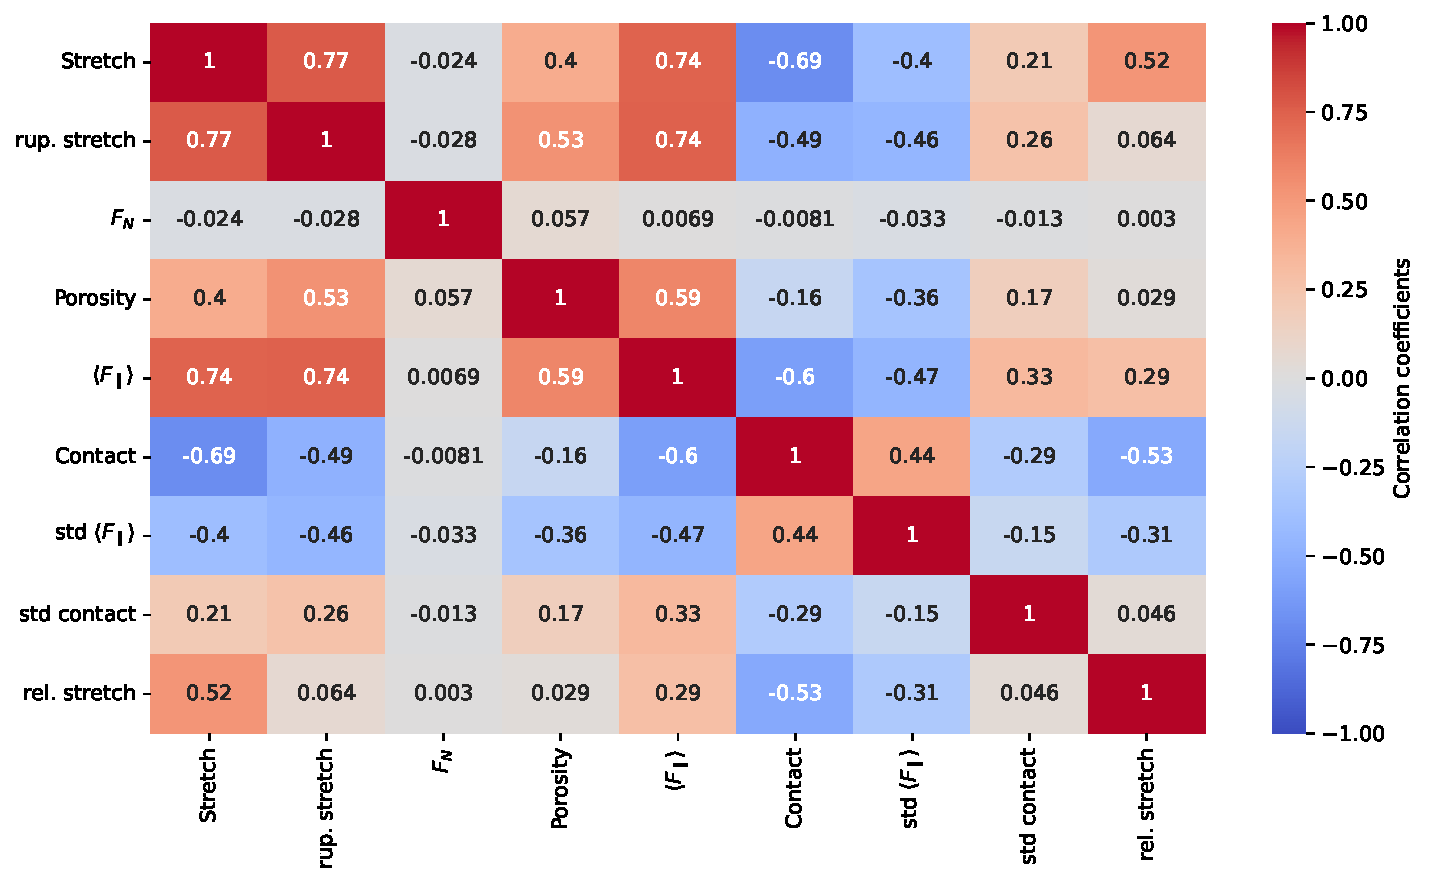
\includegraphics[width=0.81\linewidth]{figures/ML/corrcoef_matrix.pdf}
  \caption{Pearson product-moment correlation coefficients~\cref{eq:pearson} for the full datset (see~\cref{tab:dataset_summary}). Here the relative strain refers to the strain relative to the rupture strain. }
  \label{fig:corrcoef_matrix}
\end{figure}


\begin{figure}[H]
  \centering
  \begin{subfigure}[t]{0.49\textwidth}
      \centering
      \raggedleft
      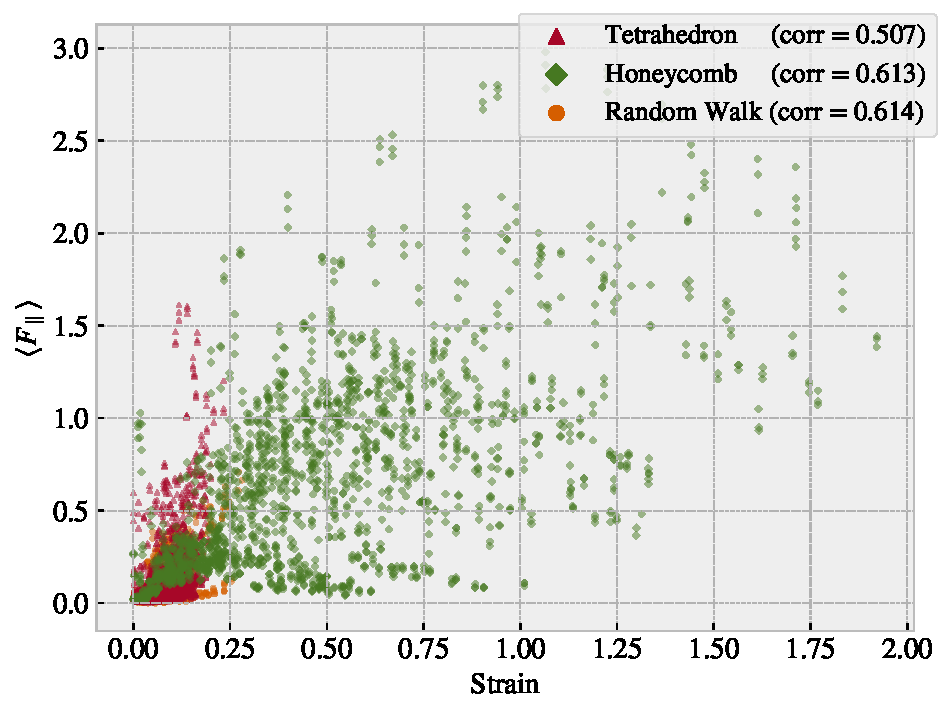
\includegraphics[width=0.82\textwidth]{figures/ML/corr_stretch_Ff.pdf}
      \caption{}
      % \label{fig:}
  \end{subfigure}
  \hfill
  \begin{subfigure}[t]{0.49\textwidth}
      \centering
      \raggedright
      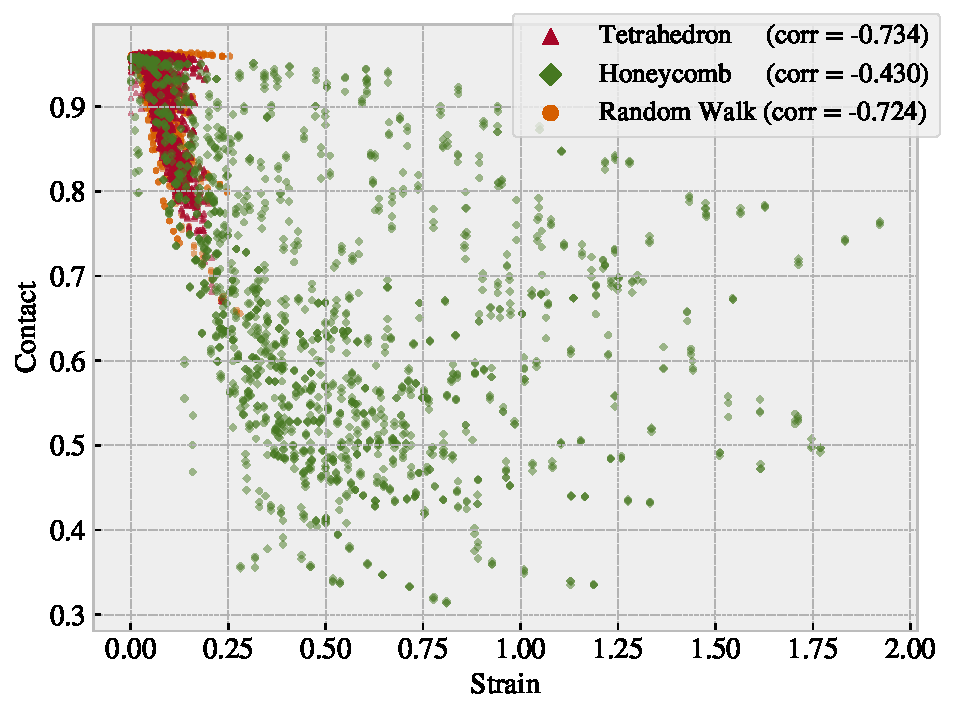
\includegraphics[width=0.82\textwidth]{figures/ML/corr_stretch_contact.pdf}
      \caption{}
      % \label{fig:}
  \end{subfigure}
  \hfill
  \begin{subfigure}[t]{0.49\textwidth}
      \centering
      \raggedleft
      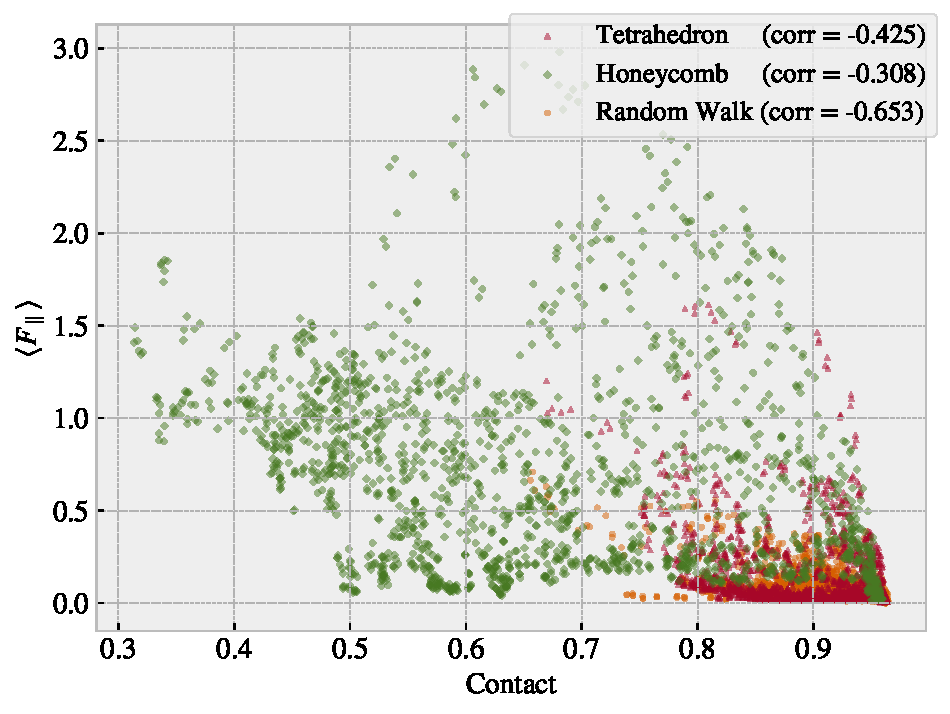
\includegraphics[width=0.82\textwidth]{figures/ML/corr_contact_Ff.pdf}
      \caption{}
      % \label{fig:}
  \end{subfigure}
  \hfill
  \begin{subfigure}[t]{0.49\textwidth}
      \centering
      \raggedright
      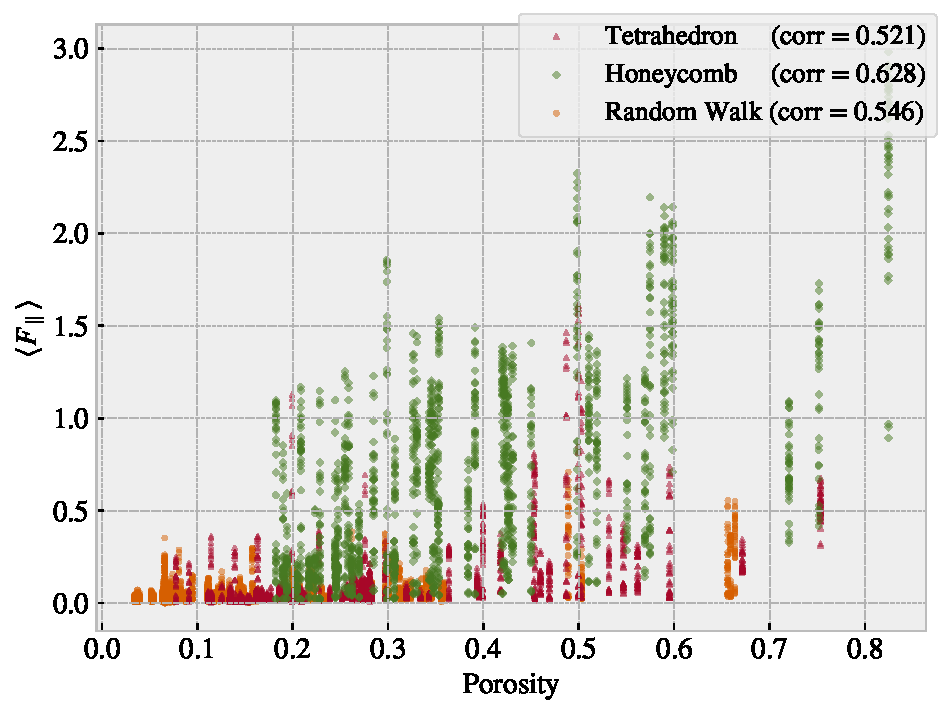
\includegraphics[width=0.82\textwidth]{figures/ML/corr_porosity_Ff.pdf}
      \caption{}
      % \label{fig:}
  \end{subfigure}
  \hfill
     \caption{Scatter plot of various dataset feature pairs for the Tetrahedron, Honeycomb and Random Walk subsets respectively. The legends include the correlation coefficient in parentheses. (a) Mean friction vs.\ strain. (b) Relative contact vs.\ strain. (c) Mean friction vs.\ relative contact. (d) Mean friction vs.\ porosity.}
     \label{fig:corr_vis}
\end{figure}


\section{Properties of interest} 
In the pilot study (\cref{chap:pilot_study}) we found promising results for the idea of achieving a negative friction coefficient under the assumption of a system with coupled normal load $F_N$ and strain $\varepsilon$. Hence, we will consider this as a main property of interest for our further exploration. We assume that the friction dependence on load is negligible $F(F_N, \varepsilon) \sim F(\varepsilon)$ in comparison to that on strain, and propose a coupling $\varepsilon = R F_N$ with linear coupling ratio $R$. From these assumptions, we can in practice substitute load for strain in the expression for the friction coefficient of our coupled system $\mu \propto \Delta F_f(\varepsilon) / \Delta \varepsilon$ as shown in~\cref{eq:mu_strain}. This justifies the search for a negative slope on the friction-strain curve since this can be related to a negative friction coefficient in our proposed coupled system. 

The remaining question is then how to evaluate the strength of this property. By
definition, the minimum (most negative) slope value would give the lowest
friction coefficient. However, two data points with a small $\Delta
\varepsilon$, corresponding to a small denominator in~\cref{eq:mu_strain}, would
potentially lead to a huge negative slope value without any significant decrease
in friction. Hence, we choose to consider the decrease in friction with
increasing strain as a better metric. Numerically we compute this by locating
the local maxima on the friction-strain curve and then evaluating the difference
to the succeeding local minima. The biggest difference corresponds to the
\textit{max drop} property which serves as our indicator for a negative friction
coefficient. In this evaluation, we do not guarantee a monotonic decrease of
friction in the strain range corresponding to the max drop, but when searching
among multiple configurations this is considered a decent strategy to highlight
configurations of interest worthy of further investigation. In addition to the
max drop property, we also consider the minimum, $\min F_{\text{fric}}$, the
maximum, $\max F_{\text{fric}}$ and the maximum difference, $\max \Delta
f_{\text{fric}} = \max F_{\text{fric}} - \min F_{\text{fric}}$ for the
friction-strain curve. The extrema of these four properties for each of the
categories: Tetrahedron, Honeycomb, Random walk and pilot study, are summarized
in~\cref{tab:data_properties}. The corresponding friction-strain profiles and
configurations are shown in~\crefrange{fig:PP_min}{fig:PP_max_drop} (excluding
the friction-strain profiles already shown in the pilot
study~\cref{chap:pilot_study}). The friction-strain profiles for the full
dataset are shown in~\cref{sec:data_stretch_profiles}. 


\begin{table}[!htb]
  \begin{center}
  \caption{Evaluation of the properties of interest for the dataset. Each table shows the top scores for each of the four properties within each of the separate data categories: Tetrahedron, Honeycomb, Random walk and pilot study (the three configurations used in the pilot study). The tables denote the names of the top candidate configurations, the relevant strain values for the property and the property values themselves. For the Tetrahedon and Honeycomb category, we compare the top candidate scores to the scores of the Tetrahedon $(7,5,1)$ and Honeycomb $(2,2,1,5)$ pattern used in the pilot study in the right-most column. }
  \label{tab:data_properties}
  \begin{tabular}{| c | c | c | c | c |} \hline
  \textbf{Tetrahedron} & Configuration & Strain & Value [nN] & Tetrahedon $(7,5,1)$ [nN]  \\ \hline
  $\min F_{\text{fric}}$ & $(3,9,4)$ &  0.0296 & 0.0067 & 0.0262 \\ \hline
  $\max F_{\text{fric}}$ & $(5,3,1)$ & 0.1391 & 1.5875 & 0.8891 \\ \hline
  $\max \Delta F_{\text{fric}}$  & $(5, 3, 1)$ & $[0.0239, 0.1391]$ & 1.5529 & 0.8603  \\ \hline
  max drop & $(5,3,1)$ & $[0.1391, 0.1999]$ & 0.8841 & 0.5098 \\ \hline
  \multicolumn{5}{c}{} \\ \hline
  \textbf{Honeycomb} & Configuration & Strain & Value [nN]  & Hon. $(2,2,1,5)$ [nN]  \\ \hline
  $\min F_{\text{fric}}$ & $(2, 5, 1, 1)$ &  0.0267 & 0.0177 & 0.0623 \\ \hline
  $\max F_{\text{fric}}$ & $(2, 1, 1, 1)$ & 1.0654 & 2.8903 & 1.5948 \\ \hline
  $\max \Delta F_{\text{fric}}$  & $(2, 1, 5, 3)$ & $[0.0856, 1.4760]$ & 2.0234 & 1.5325 \\ \hline
  max drop & $(2, 3, 3, 3)$ & $[0.5410, 1.0100]$ & 1.2785 & 0.9674\\ \hline
  \multicolumn{5}{c}{} \\ \cline{1-4}
  \textbf{Random walk} & Configuration & Strain & Value [nN] & \multicolumn{1}{c}{} \\ \cline{1-4}
  $\min F_{\text{fric}}$ & 12 &  0.0562 & 0.0024& \multicolumn{1}{c}{} \\ \cline{1-4}
  $\max F_{\text{fric}}$ & 96 & 0.2375 & 0.5758 & \multicolumn{1}{c}{} \\ \cline{1-4}
  $\max \Delta F_{\text{fric}}$  & 96 & $[0.0364, 0.2375]$ & 0.5448 & \multicolumn{1}{c}{} \\ \cline{1-4}
  max drop & 01 & $[0.0592, 0.1127]$ & 0.1818 & \multicolumn{1}{c}{} \\ \cline{1-4}
  \multicolumn{5}{c}{} \\ \cline{1-4}
  \textbf{Pilot study} & Configuration & Strain & Value [nN]  & \multicolumn{1}{c}{} \\ \cline{1-4}
  $\min F_{\text{fric}}$ & No cut & 0.2552 & 0.0012 & \multicolumn{1}{c}{} \\ \cline{1-4}
  $\max F_{\text{fric}}$ & Hon. $(2,2,1,5)$ & 0.7279 & 1.5948 & \multicolumn{1}{c}{} \\ \cline{1-4}
  $\max \Delta F_{\text{fric}}$  & Hon. $(2,2,1,5)$ & 0.7279 & 1.5325 & \multicolumn{1}{c}{} \\ \cline{1-4}
  max drop & Hon. $(2,2,1,5)$ & $[0.7279, 1.0463]$ & 0.9674 & \multicolumn{1}{c}{} \\ \cline{1-4}
\end{tabular}
\end{center}
\end{table}

From the property comparison in~\cref{tab:data_properties}, we find that both the
Tetrahedron and Honeycomb subsets contain improved candidates for each of the
property scores in comparison to the Tetrahedron $(7,5,1)$ and Honeycomb
$(2,2,1,5)$ examined in the pilot study. Overall, the Honeycomb pattern type is
resulting in the highest scores for the maximum properties while the minimum
friction is still achieved by the non-cut sheet. This latter observation
confirms the findings of the pilot study since our dataset does not provide any
indication that friction can be reduced for a Kirigami sheet under strain.
However, the improvement in the remaining properties indicates that the dataset
contains valuable information that can provide a direction for further optimization of
the maximum properties. Considering the Random walk we find that the max
property scores are generally lower than those of the Tetrahedron and Honeycomb
patterns. However, since these are found to be on a comparable order of
magnitude we argue that these contribute relevant information for the
frictional dependency to Kirigami configurations. The Random walk patterns
exhibit greater diversity compared to the other patterns and therefore provide
some immediate insights into which structures can be associated with each of the
properties of interest. For the $\min F_{\text{fric}}$ top candidates
(\cref{fig:PP_min}) we find that the Random walk candidate has a rather low cut
density (low porosity) and vertical cuts. Since these cuts run parallel to
the stretching direction one can hypothesize that this minimizes the induced
buckling effect which agrees with the relatively flat contact-strain curve. For the minimum candidate of the Tetrahedron pattern, we also observe
a low decrease in contact area, and in both these cases this corresponds with a
seemingly flat friction-strain curve as well. When considering the remaining
friction-strain curves throughout~\crefrange{fig:PP_min}{fig:PP_max_drop} we
find that a rising friction-strain curve is always seen together with a
declining contact-strain curve. This supports the general observation of a
correlation between the strain-induced friction effects and the contact area.
When looking at the $96\text{th}$ Random walk pattern, which is the top
candidate for both the $\max F_{\text{fric}}$ (\cref{fig:PP_max}) and $\max
\Delta f_{\text{fric}}$ (\cref{fig:PP_max_diff}) properties, we find a rather
porous configuration with mainly horizontal-orientated cuts. This has some
structural reminiscence with the general shape of the Honeycomb pattern.
Finally, for the Random walk max drop candidate, Random walk pattern 01, we do see a
small drop in friction. Although, this is not as significant as seen for the
Tetrahedron and Honeycomb candidates. We notice that the configuration contains
some slanted cuts which might be reminiscent of parts of the general Tetrahedron
pattern. 




\begin{figure}[H]
  \centering
  \begin{subfigure}[t]{1\textwidth}
      \centering
      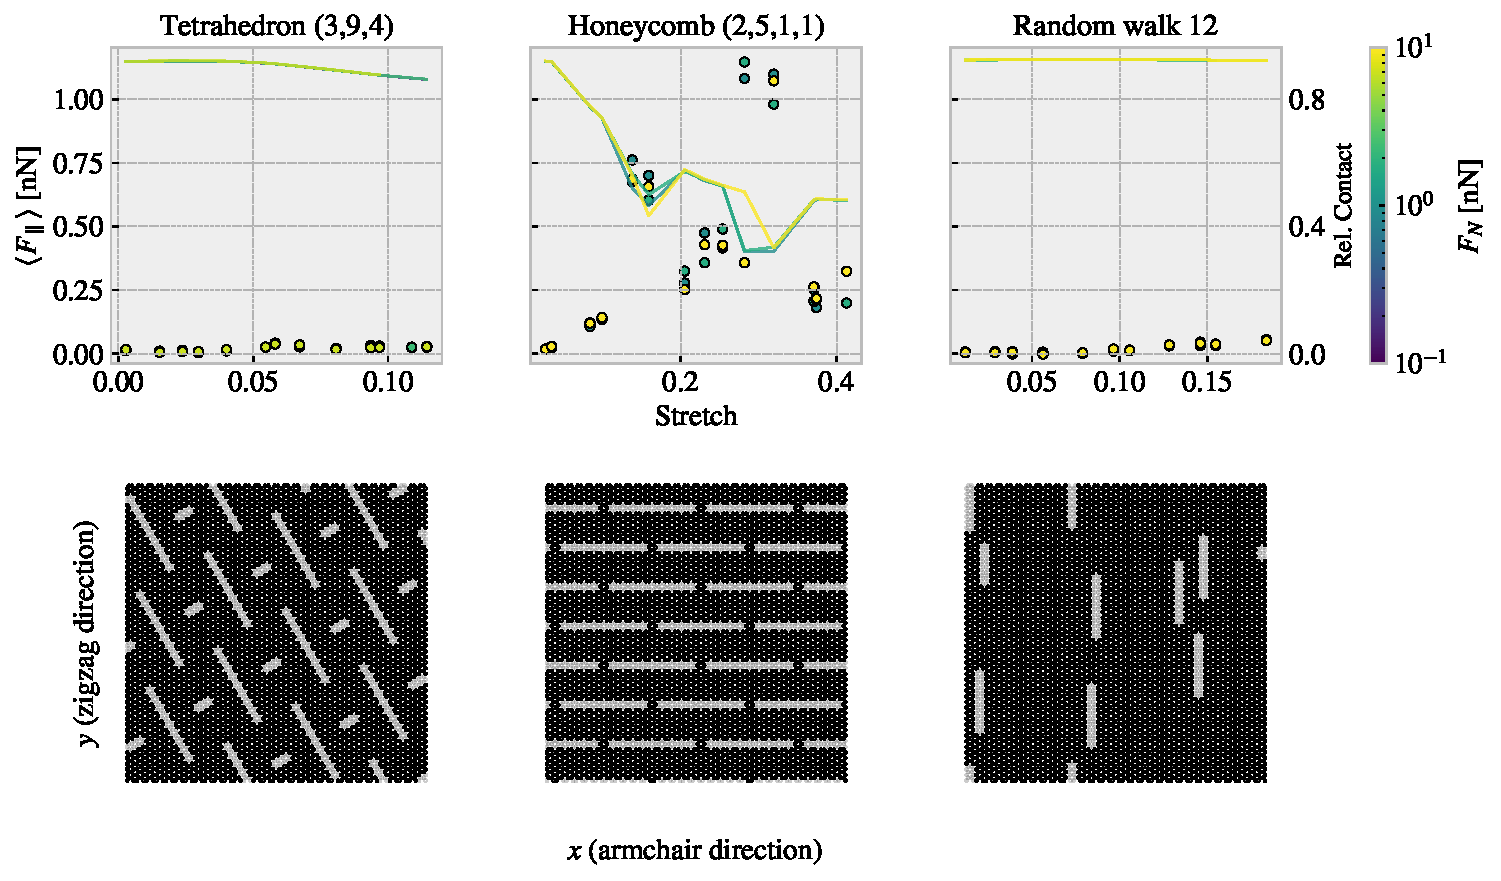
\includegraphics[width=\linewidth]{figures/stretch_profiles/PP_min.pdf}
      \caption{Minimum friction ($\min F_{\text{fric}}$).}
      \label{fig:PP_min}
  \end{subfigure}
  \hfill
  \vspace{1cm}
  \begin{subfigure}[t]{1\textwidth}
      \centering
      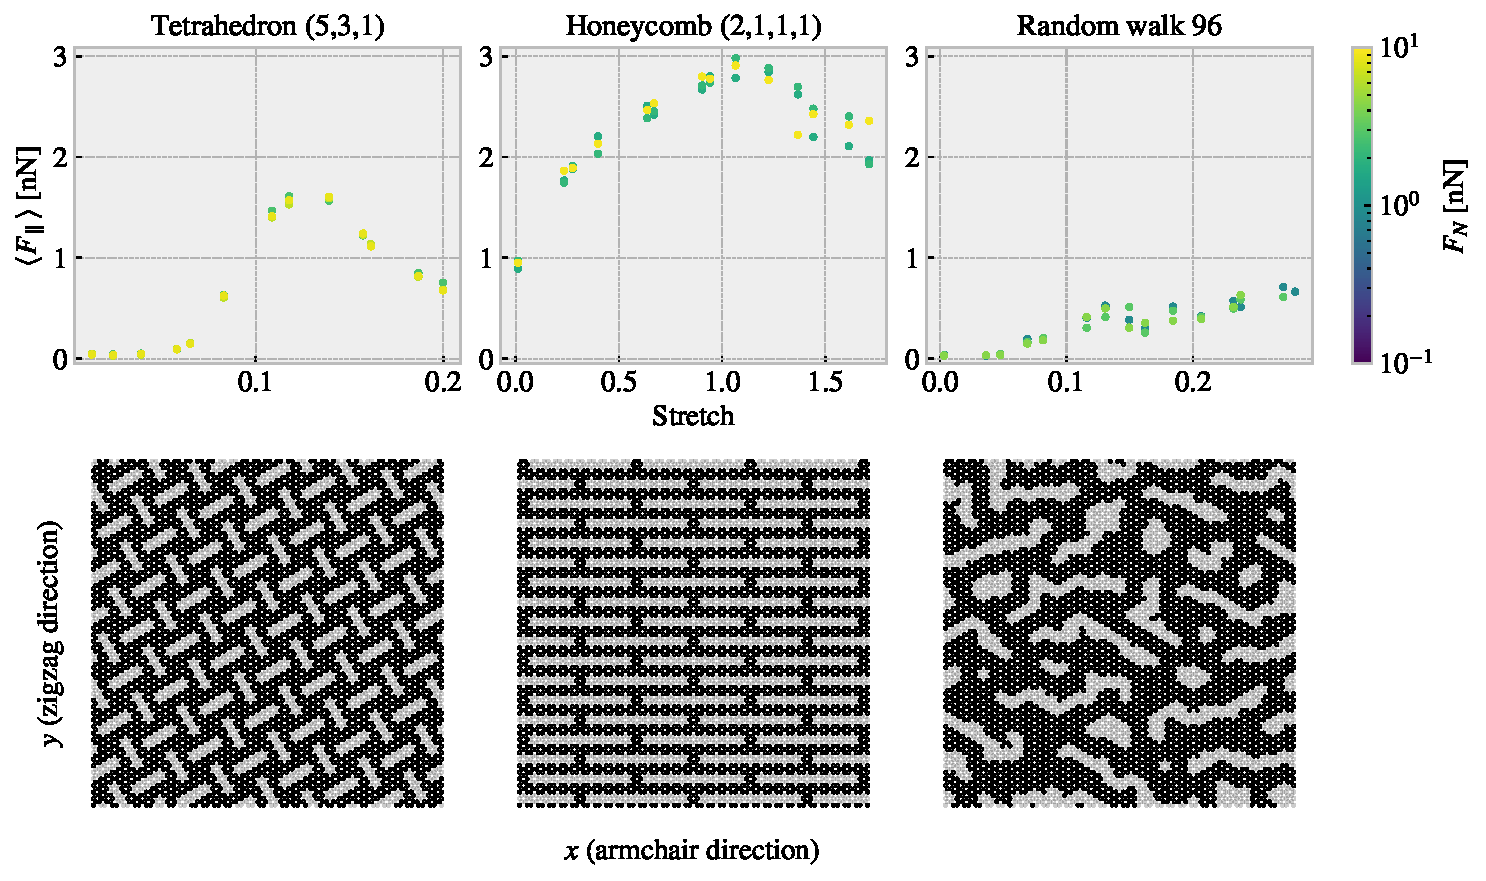
\includegraphics[width=\linewidth]{figures/stretch_profiles/PP_max.png}
      \caption{Maximum friction ($\max F_{\text{fric}}$)}
      \label{fig:PP_max}
  \end{subfigure}
  \hfill
  \caption{(The figure continues on the next page)}
\end{figure}

\begin{figure}[H]\ContinuedFloat
  \centering
  \begin{subfigure}[t]{1\textwidth}
      \centering
      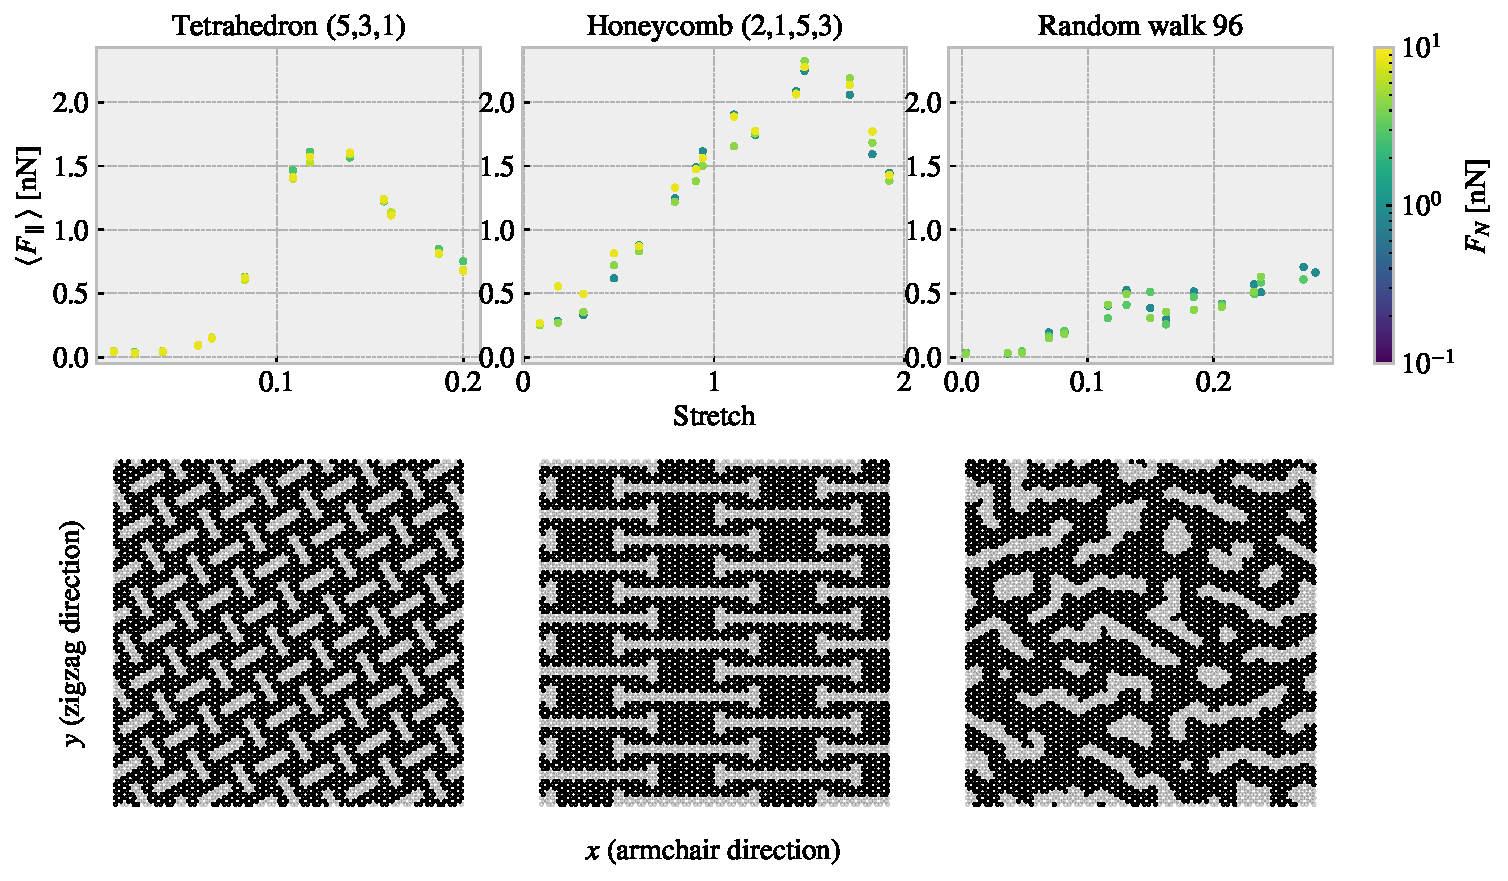
\includegraphics[width=\linewidth]{figures/stretch_profiles/PP_max_diff.png}
      \caption{Maximum friction difference ($\max \Delta F_{\text{fric}}$).}
      \label{fig:PP_max_diff}
  \end{subfigure}
  \hfill
  \vspace{1cm}
  \begin{subfigure}[t]{1\textwidth}
      \centering
      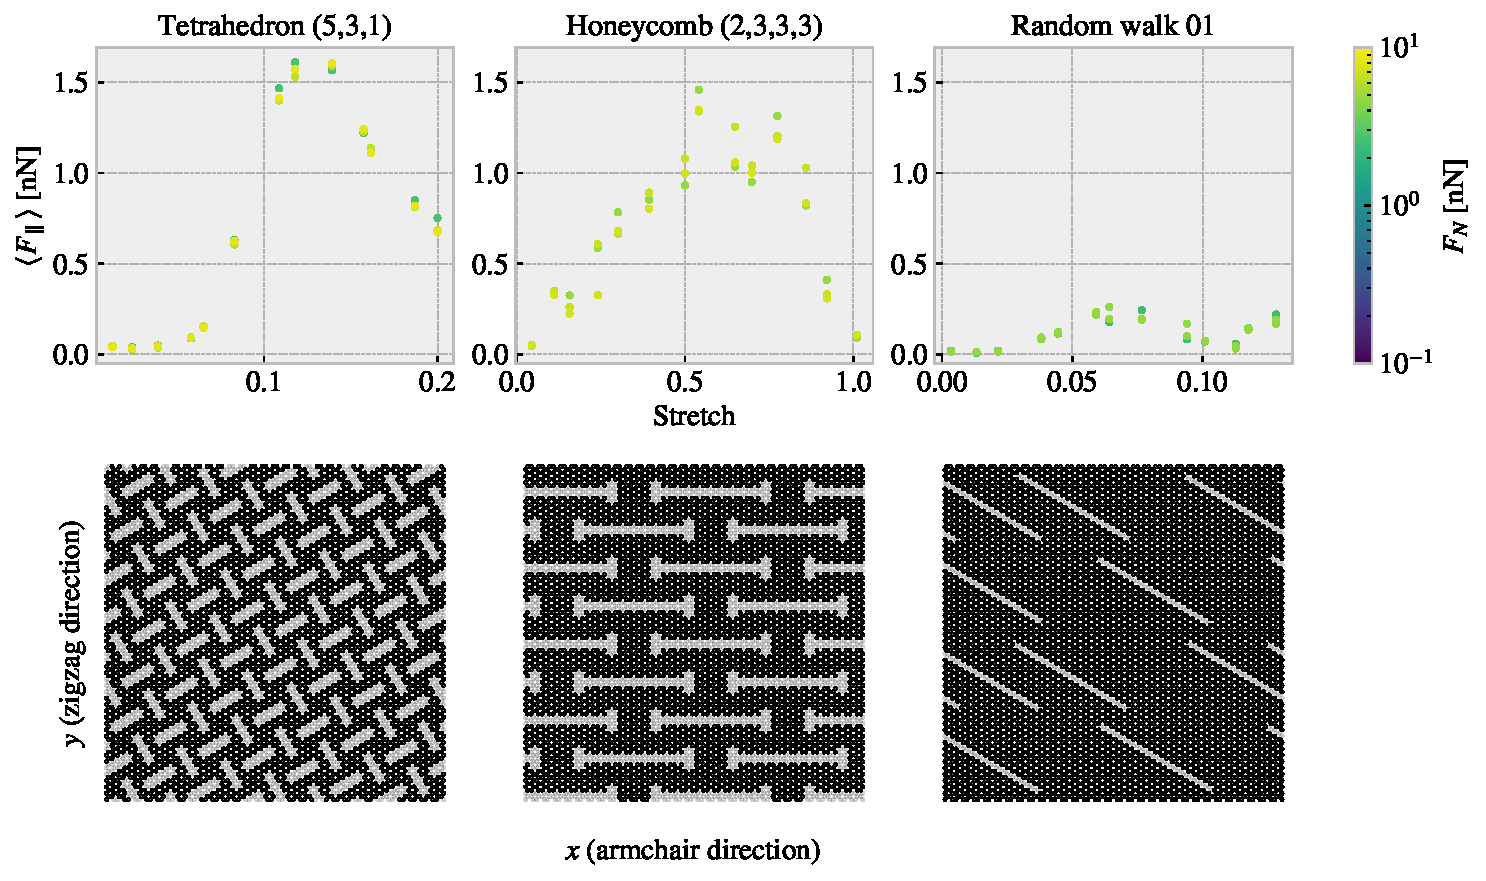
\includegraphics[width=\linewidth]{figures/stretch_profiles/PP_max_drop.png}
      \caption{Maximum drop in friction (max drop).}
      \label{fig:PP_max_drop}
  \end{subfigure}
  \hfill
  \caption{Illustration of the top candidates within each of the four properties of interest. The upper row shows the friction-strain curve with dotted points (friction value on the left y-axis) and the contact-strain curve with a solid line (relative contact value on the right y-axis). The bottom row shows the corresponding Kirigami patterns. (a) Minimum friction ($\min F_{\text{fric}}$). (b) Maximum friction ($\max F_{\text{fric}}$). (c) Maximum friction difference ($\max \Delta F_{\text{fric}}$).  (d) Maximum drop in friction (max drop). }
  \label{fig:PP}
\end{figure}


\section{Machine learning}\label{eq:ML}
Given the \acrshort{MD}-based dataset presented in the previous section, containing Honeycomb, Tetrahedron and Random walk geometries, we investigate the possibilities of training a machine learning model to predict the friction behavior from a given Kirigami configuration, strain and load. 

\subsection{Architecture}
Due to the spatial dependencies in the Kirigami configurations, we use a convolutional neural network (\acrshort{CNN}). Similar studies which predict mechanical properties for graphene sheets have used a VGGNet style of network, Hanakata et al.~\cite{PhysRevLett.121.255304, PhysRevResearch.2.042006} and Wan et al.~\cite{graphene/hBN}, which we adopt for this study as well. The VGGNet-16 architecture illustrated in~\cref{fig:VGGNet16} shows the key features that we will include:
\begin{itemize}
  \item The image is processed through a series of $3 \times 3$ convolutional filters (the smallest size capable of capturing spatial dependencies) using a stride of 1 with an increasing number of channels throughout the network. We use zero padding to conserve the spatial size during a convolution. Each convolutional layer is followed by a ReLU activation function. 
  \item The spatial dimensions are reduced by a max pooling layer, filter size $2 \times 2$ and a stride of 2, which halves the spatial resolution each time. 
  \item The latter part of the network consists of a fully connected part using the ReLu activation as well. The transition from the convolutional to the fully connected part is achieved by applying a filter with the same dimensions as the last convolutional feature map. This essentially performs a linear mapping from the spatial output to the fully connected layer where the number of channels corresponds to the nodes in the first fully connected layer.
\end{itemize}

\begin{figure}[!htb]
  \centering
  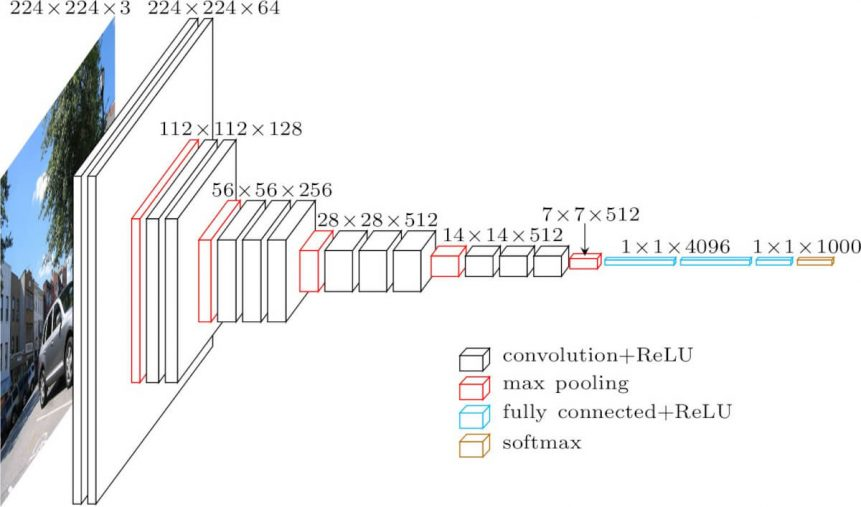
\includegraphics[width=0.6\linewidth]{figures/ML/VGGNet16.jpg}
  \caption{Illustration of the convolutional network architecture for the VGGNet-16 proposed by K.\ Simonyan and A.\ Zisserman~\cite{simonyan2015deep}. Reproduced from~\cite{VGGNet_16_image}.}
  \label{fig:VGGNet16}
\end{figure}

We deviate from the VGGNet-16 architecture by including batch normalization and restricting ourselves to setting up the convolutional part of the network in terms of the convolutional block (Convolution $\to$ Batch normalization $\to$ ReLU $\to$ Max pooling). Similarly, we define a fully connected block by two elements (Fully connected $\to$ ReLU) which match the VGGNet model. Hanakata et al.\ and Wan et al.\ used a similar architecture with the parameters 
\begin{align*}
  \text{Hanakata et al.~\cite{PhysRevLett.121.255304}} & \qquad C16 \ C32 \ C64 \ D64, \\ 
  \text{Wan et al.~\cite{graphene/hBN}} & \qquad C16 \ C32 \ D32 \ D16,
\end{align*}
where $C$ denotes a convolutional block with the number denoting the number of channels, and $D$ a fully connected (dense) block with the number denoting the number of nodes. For the purpose of determining a suiting complexity for the architecture, we adopt the approach by Wan et al.~\cite{graphene/hBN} who used a ``staircase'' pattern for combining the convolutional and fully connected blocks. By defining a starting number of channels $S$ for the first convolutional layer and a network depth $D$ we fill the first half of the network layers with convolutional blocks, doubling in channel number for each layer, and the latter half with fully connected blocks halving the number of nodes in a reverse pattern. For instance, the architecture $S4D8$ will take the form
\begin{align}
  \text{Input} \to \underbrace{\overbrace{C4}^{S \ = \ 4}C8 \ C16 \ C32 \ D32 \ D16 \ D8 \ D4}_{D \ = \ 8} \to \text{Output}.
  \label{eq:staircase_example}
\end{align} 
This provides a simple description where $S$ and $D$ can be varied systematically for a grid search over architecture complexity. 


\subsection{Data handling}
\subsubsection{Input}
We use three variables as input: Kirigami configuration, strain of the sheet
and applied normal load. The Kirigami configuration is given as a two-dimensional binary matrix while the strain and load are both scalar values. This gives rise to two different options for the data structure:
\begin{enumerate}
  \item Expand the scalar values (strain and load) into 2D matrices of the same
  size as the Kirigami configuration matrix by copying the scalar value to all matrix coordinates. This can then be merged into an image of three channels used as a single input.  
  \item Pass only the Kirigami configuration through the convolutional part of the network and introduce the remaining scalar values directly into the fully connected part of the network halfway in. 
\end{enumerate}
Both options utilize the same data, but the latter option is more directed toward independent processing of the data while the first makes for an intertwined use of the configuration, strain and load input. We implemented both options but found immediately that option 1 was producing the most promising results during short training tests, and thus we settled for this data structure. 

\subsubsection{Output}
For the output, we are mainly concerned with mean friction and the rupture
detection. In combination, these values will make the model able to produce a friction-strain curve with an estimated stopping point as well. However, in order to retain the option to explore other relations in the data we include the maximum friction, relative contact, porosity and rupture strain in the output as well. Notice that we weigh the importance of these output variables differently in the loss as described in~\cref{sec:loss}. 


\subsubsection{Data augmentation}
In order to increase the utility of the available data one can introduce data
augmentation. For most classification tasks this usually includes distortions
such as color shifts, zoom, reflect etc. However, such distortions are only valid
since the classification network should still classify a cat as a cat even
though it is suddenly a bit brighter or flipped upside down. For our problem, we
can only use augmentation that matches a physical symmetry. Such a symmetry
exists for reflection across the y-axis, and thus we perform this transformation
with a 50\% chance for both training and validation data. We cannot use a reflection
across the x-axis as the sheet is sliding in a positive y-direction. Such a
transformation would correspond to a change in the sliding direction which we
cannot expect to be fully symmetric. 


\subsection{Loss}\label{sec:loss}
The output contains two different types of variables: scalar values and a binary value (rupture). For the scalar values we use the mean squared error~\cref{eq:MSE} and for the binary output we use binary cross entropy~\cref{eq:BSE}. We calculate the total loss as a weighted sum of the loss associated with
each output
\begin{align*}
  L_{tot} = \sum_{o} W_o\cdot L_o.
\end{align*}
We choose the weights $W_o$ to be $1/2$ for the mean friction and $1/10$ for the
remaining 5 output variables, thus sharing the loss evenly for the remaining 50\% of the weight. During the introductory phase of the model implementation, we tried different settings for these weights, but we found that the results varied little. Hence, we concluded that this was of minor importance and we settled on the values defined above.

\subsection{Hypertuning}
For the hypertuning we focus on architecture complexity, learning rate, momentum and weight decay. We use the ADAM optimizer with the initial default values of $\beta_1 = 0.9, \beta_2 = 0.999$ and zero weight decay, for which we will vary momentum $\beta_1$ and weight decay in the hypertuning. We use a batch size of 32 and train the model for a maximum of 1000 epochs while storing the best model based on the validation scores.
Since the learning rate is considered to be one of the most important hyperparameters we will determine a suitable choice for the learning rate using the learning rate range test for each of the two grid searches:
\begin{enumerate}
  \item Architecture complexity grid search of $S$ vs.\ $D$ with individually chosen learning rates for each complexity combination.
  \item Momentum vs.\ weight decay grid search with learning range chosen with regard to each momentum setting.
\end{enumerate}
We consider first the architecture complexities in the range $S \times D =
\{2,4,8,16,32,64,128,256\} \times \{4,6,8,10,12,14\}$. For each architecture
complexity, we perform an initial learning rate range test and determine the suitable choice for the learning rate as the point for which the validation loss decreases most rapidly. The learning rate is increased exponentially within the range \num{e-7} to 10 with increments for each training batch iteration. This is done for a single epoch where a batch size of 32 yields a total of 242 possible increments. This corresponds to an exponent increment of approximately $1/30$ giving a relative increase $10^{1/30} \sim 108\%$ per batch iteration. The learning rate range test is presented in~\cref{fig:LR_range} for various model complexities. We notice that the suggested learning rate decreases with an increasing number of model parameters. This decrease is further independent of the specific relationship between $S$ and $D$.

\begin{figure}[H]
  \centering
  \begin{subfigure}[t]{0.49\textwidth}
      \centering
      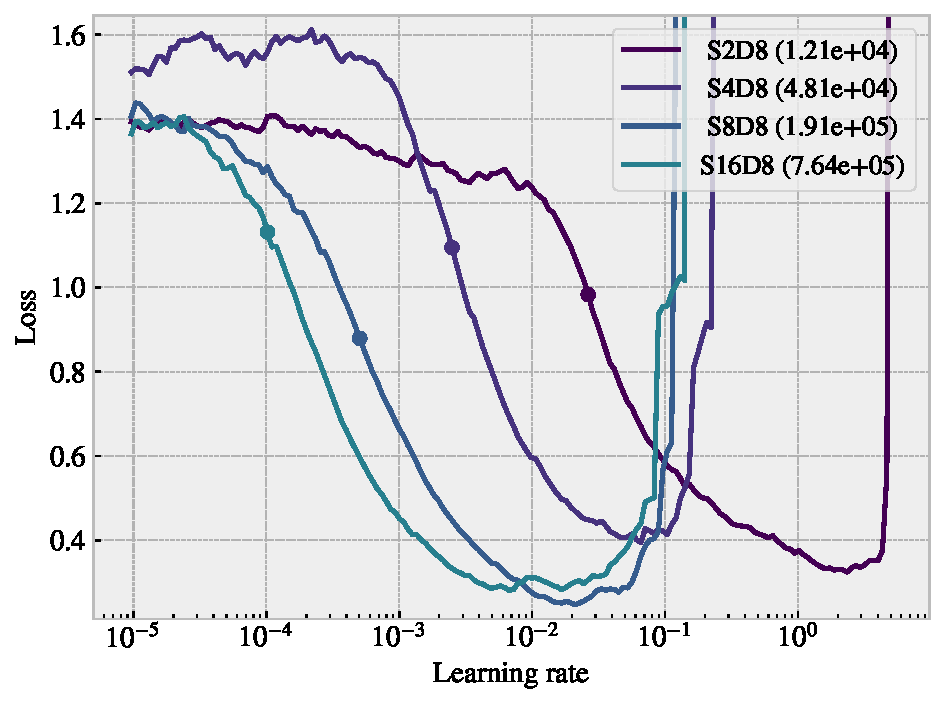
\includegraphics[width=\textwidth]{figures/ML/LR_range_specific.pdf}
      \caption{}
      % \label{fig:}
  \end{subfigure}
  \hfill
  \begin{subfigure}[t]{0.49\textwidth}
      \centering
      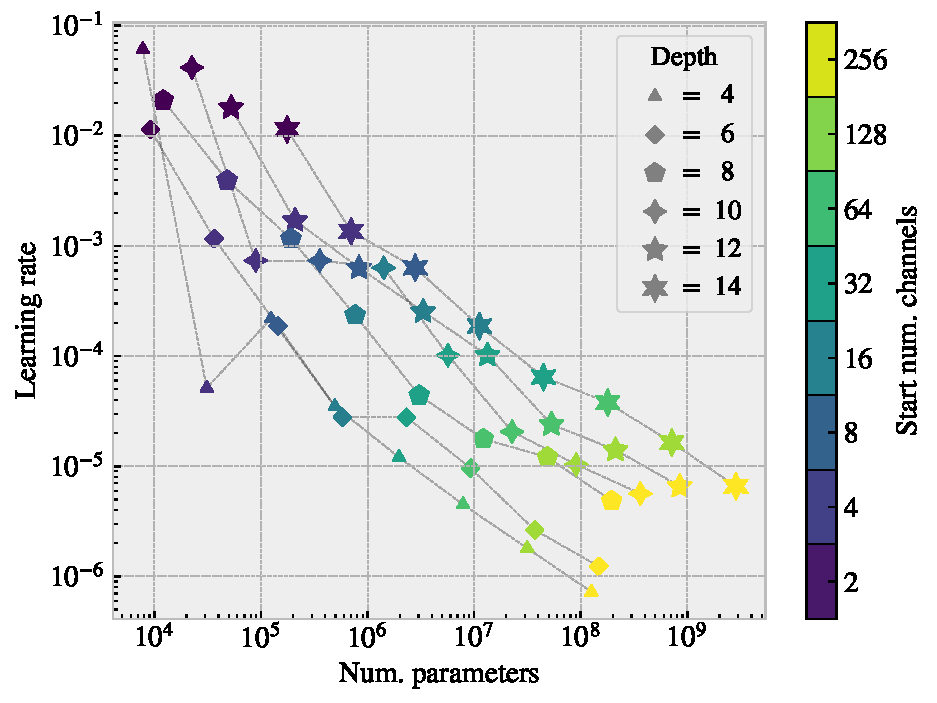
\includegraphics[width=\textwidth]{figures/ML/LR_range_full.pdf}
      \caption{}
      % \label{fig:}
  \end{subfigure}
  \hfill
  \caption{Learning rate range test for various model complexities. We increase the learning rate exponentially from \num{e-7} to 10 during one epoch corresponding to an exponent increment of roughly $1/30$ per batch iteration. (a) A few examples of the validation loss as a function of the learning rate. The exemplary architectures are S[2, 16]D8 with the corresponding number of model parameters shown in parentheses in the legend. The dots indicate the suggested learning rate at the steepest decline of the validation loss. (b) The full results showing the suggested learning rates depending on the number of model parameters with color coding differentiating the number of start channels $S$ and marker types differentiating different model depths $D$. }
  \label{fig:LR_range}
\end{figure}


With the use of the suggested learning rates from~\cref{fig:LR_range} we perform
a grid search over the corresponding $S$ and $D$ parameters. We evaluate both
the validation loss and the mean friction $R^2$ score for the validation data which is shown in~\cref{fig:A_search_perf} together with the best epoch and the number of model parameters. Additionally, we evaluate the mean friction $R^2$ score for a selected set of configurations. This set consists of the top 10 configurations with respect to the max drop property for the Tetrahedron and Honeycomb patterns respectively. This is done as a way of evaluating the performance on the non-linear friction-strain curves which we find to be the more difficult trend to capture. The selected evaluation is shown in~\cref{fig:A_search_compare}. Note that these configurations are already a part of the full dataset and thus the data points related to these configurations are most likely present in both the training and the validation data set. Hence, the performance must be considered in conjunction with the actual validation performance in~\cref{fig:A_search_perf}.


%%

%% 

From the validation scores in~\cref{fig:A_search_perf}, looking at both the loss
and the $R^2$ scores, we find that models S(8-32)D(8-12) generally give the best
performance. When considering at the best epoch, we find that models of low depth
result in a later best epoch in the range $\sim [800, 1000]$, in comparison to
models of high depth yielding the best epoch in the range $\sim [300, 600]$.
This indicates a transition from underfitting to overfitting of the model since
the best validation scores are found earlier in the training process. However,
since our training stores the best model during training, we do not have to
worry too much about overfitting. Nonetheless, we can take this transition as a
sign that our search is conducted in an appropriate complexity range. When
consulting the evaluation on the selected sets in~\cref{fig:A_search_compare} we
find significantly lower $R^2$ scores, especially for the Tetrahedron pattern.
This observation indicates that the prediction of these configurations is more
difficult, especially when considering that some of these data points are already included in the
training data. While the peak $R^2$ value for the validation score
in~\cref{fig:A_search_perf} was found for the model S16D10 model (98.23 \%) the
selected set test shows a slight preference for more complexity in the model. In
the Tetrahedron selected set grid search, we find the best model to be S32D12,
with an $R^2$ score of $\sim 87 \%$. This model choice is more or less
compatible with the overall performance since it is among the top candidates for
the $R^2$ score and loss in~\cref{fig:A_search_perf} and the $R^2$ score for the
selected Honeycomb set in~\cref{fig:A_search_compare} as well. Hence, we settle
for this architecture. 


\begin{figure}[!htb]
  \centering
  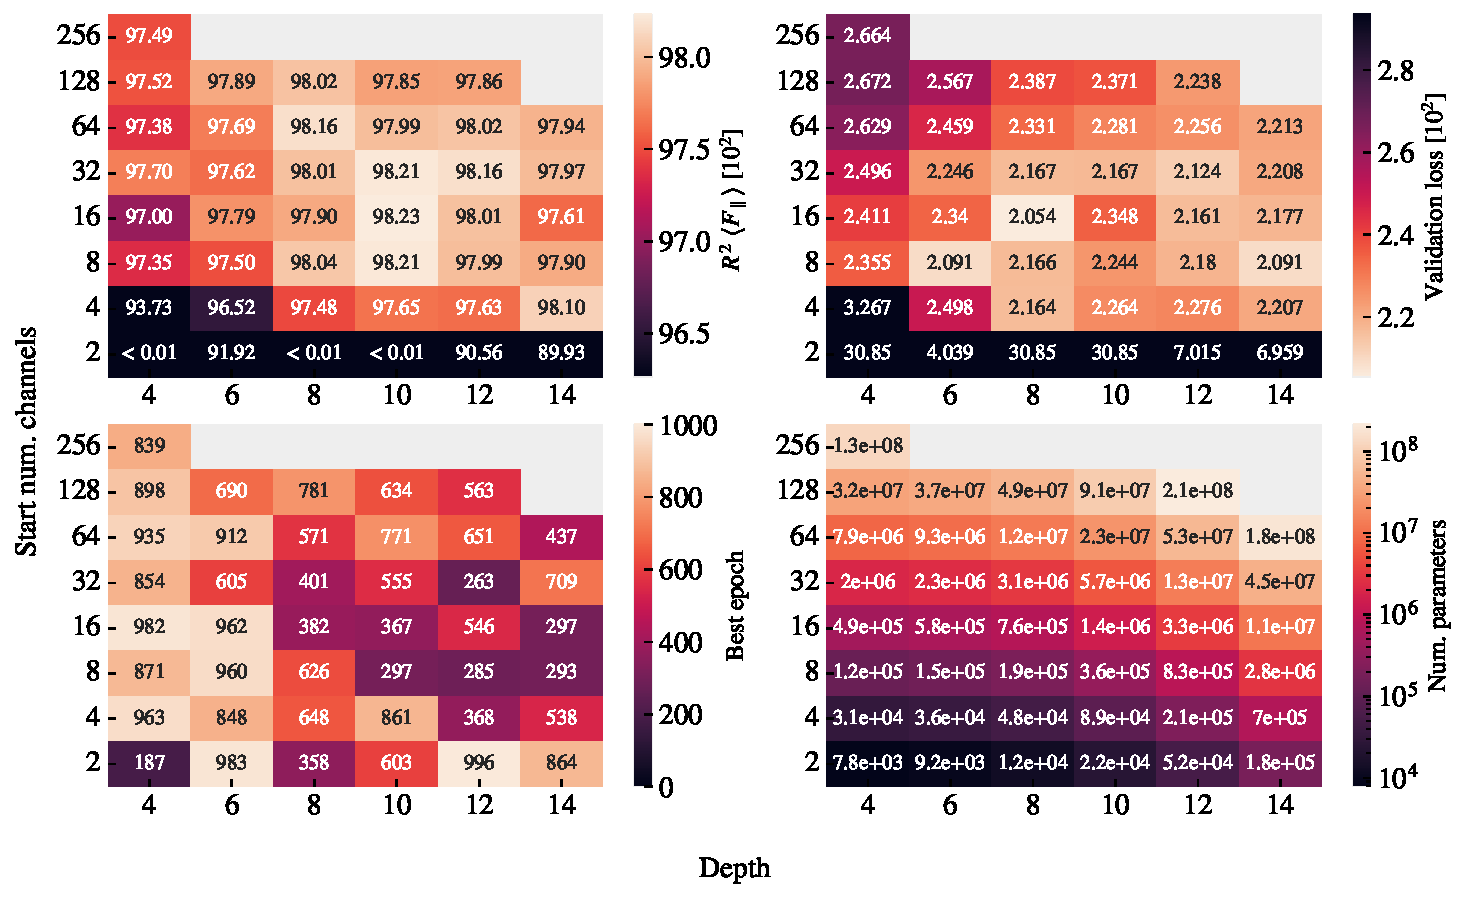
\includegraphics[width=\linewidth]{figures/ML/A_search_perf.pdf}
  \caption{Architecture complexity grid search using a staircase-like VGGNet structure. The x-axis denotes the number of layers in the network (Depth) and the y-axis is the starting number of channels. See~\cref{eq:staircase_example} for an example of the staircase architecture. For each architecture complexity, we evaluate the friction mean $R^2$ validation score (top left), the validation loss (top right), the best epoch stored based on validation scores (bottom left) and the number of model parameters (bottom right).}
  \label{fig:A_search_perf}
\end{figure}  


We note that the theoretical receptive field for the last
convolutional layer (layer 6) is $13 \times 13$ according to~\cref{eq:receptive_field}, and thus each node in the first fully connected
layer does not connect to the entirety of the $62\times106$ input image. Hence,
some spatial dependence will have to be encoded in the fully connected part as
well, and we note that an enlargement of the receptive field might serve as an interesting suggestion for an improvement of the model in further studies. One possible method is to increase the stride or use dilated convolutions.





\begin{figure}[!htb]
  \centering
  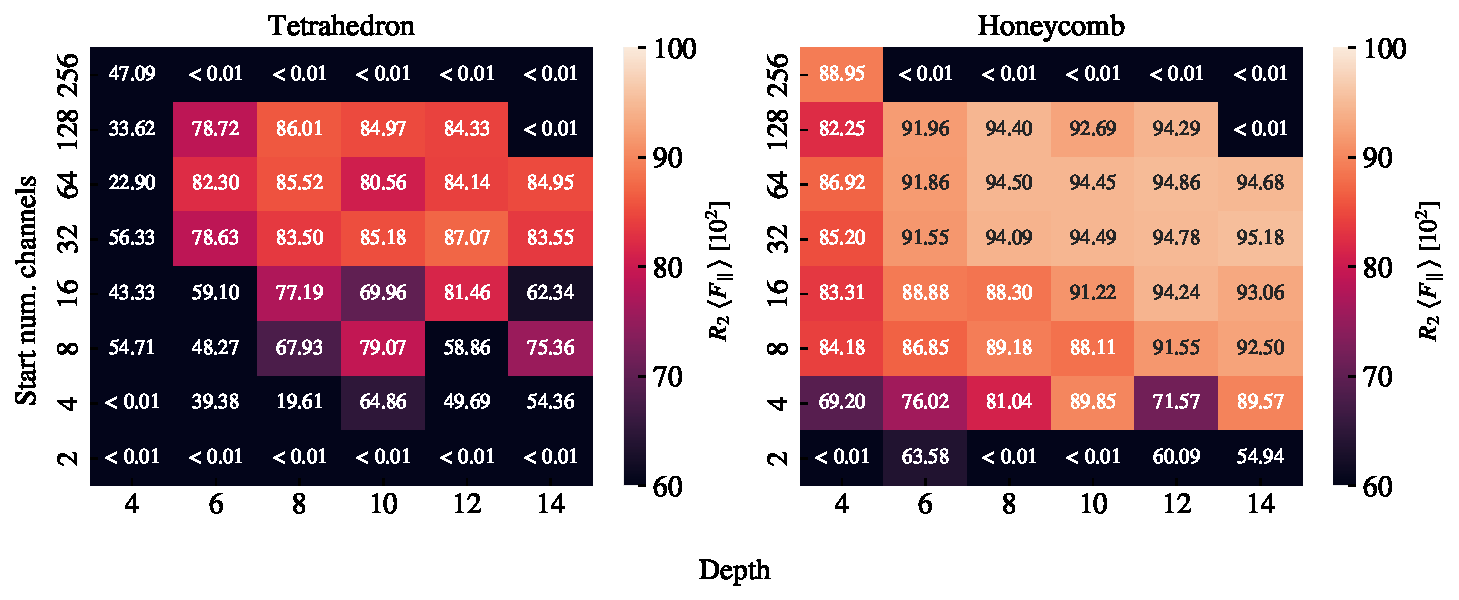
\includegraphics[width=\linewidth]{figures/ML/A_search_compare_perf}
  \caption{Architecture grid search similar to that of~\cref{fig:A_search_perf} on a selected set of configurations. The selected set consists of the top 10 candidates for the max drop property for the Tetrahedron and Honeycomb categories in the dataset respectively.}
  \label{fig:A_search_compare}
\end{figure}  



Next, we consider momentum $m$ and weight decay $\lambda$ in the range $m \in
[0.85, 0.99]$ and $\lambda \in [0, \num{e-2}]$. For each choice of momentum, we
perform a learning rate range test. We propose two learning rate schemes: A
constant learning rate scheme as used until this point and a one-cycle policy cyclic scheme. In the cyclic scheme, we set a maximum bound for which the learning rate starts from a factor $1/20$ of the maximum bound, increases toward the maximum bound during the first $30\%$ of training and decreases toward a factor \num{e-4} of the maximum bound for the remaining 70\% of training. The increase
and decrease are done by a cosine function. We let the momentum follow an inverse cycle with a minimum of $m = 0.80$ and a maximum corresponding to the momentum value being tested. The suggested learning rate for the
constant learning rate scheme is once again determined by the steepest slope on
the learning range test loss curve while the maximum bound used for the
cyclic scheme is determined as the point just before divergence. We find that
the minimum point on the loss curve is a suitable choice that approaches the
diverging point without getting too close and causing instabilities in the
training. The learning rate range test for momentum is shown
in~\cref{fig:LR_range_mom}. We observe generally that a higher momentum
corresponds to a higher suggested learning rate for both schemes. Using these
results we perform a grid search of momentum and weight decay. We examine again
the validation loss and validation mean friction $R^2$ score in addition to the
friction mean $R^2$ score for the selected set of Tetrahedron and Honeycomb
patterns. This is shown for the constant learning rate scheme
in~\cref{fig:mom_weight_search_constant} and for the cyclic scheme
in~\cref{fig:mom_weight_search_cyclic}.


\begin{figure}[!htb]
  \centering
  \begin{subfigure}[t]{0.49\textwidth}
      \centering
      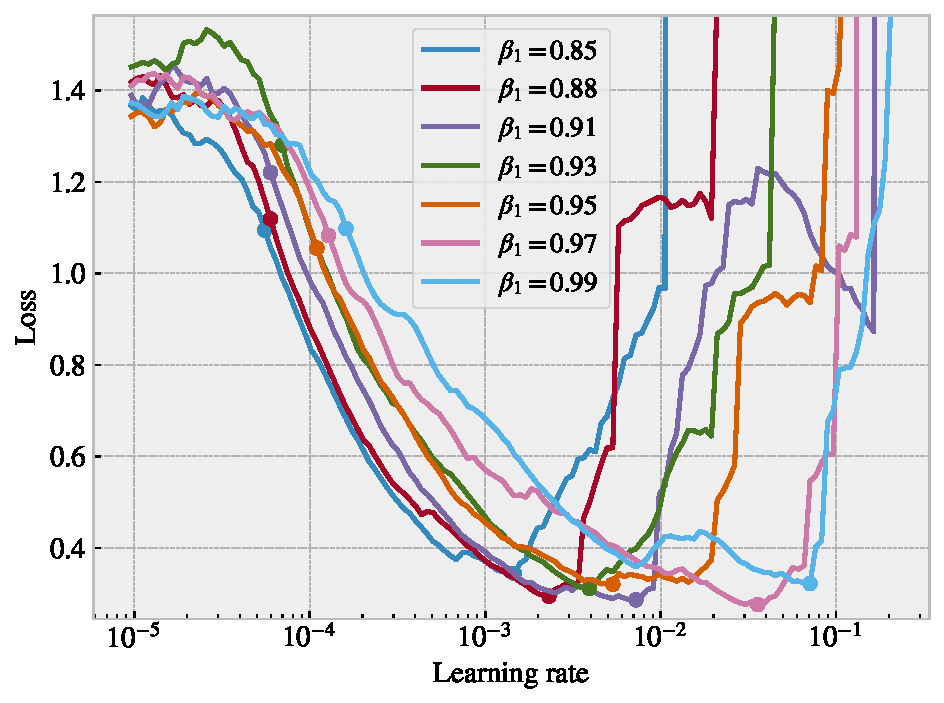
\includegraphics[width=0.95\textwidth]{figures/ML/LR_momentum_test_a.pdf}
      \caption{}
      % \label{fig:}
  \end{subfigure}
  \hfill
  \begin{subfigure}[t]{0.49\textwidth}
      \centering
      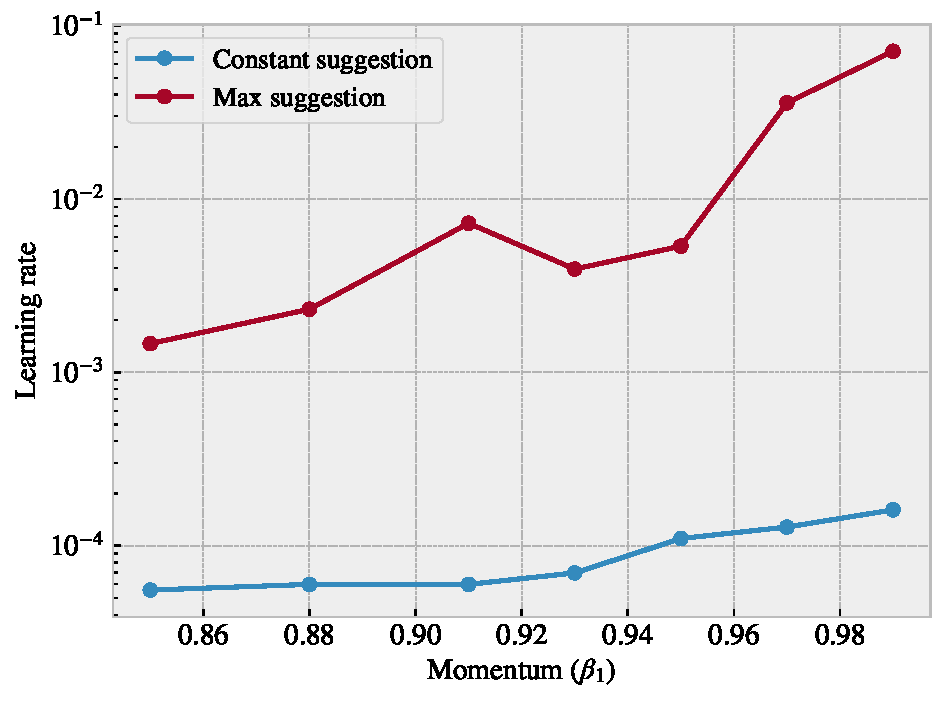
\includegraphics[width=0.95\textwidth]{figures/ML/LR_momentum_test_b.pdf}
      \caption{}
      % \label{fig:}
  \end{subfigure}
  \hfill
  \caption{Learning rate range test for different momentum values $m$. (a) The validation loss for an exponentially increasing learning rate from \num{e-7} toward 10 with increments for each batch iteration during 1 epoch (yielding a total of 242 possible increments). As the curve diverges the test is halted. The dots on the validation loss vs.\ learning rate curve represent the steepest decline (at a lower learning rate) as an estimate for the constant learning scheme, and the minimum (at a higher learning rate) as an estimate for the maximum bound for the cyclic learning rate scheme. (b) The corresponding learning rate suggestion for the constant learning rate scheme and the maximum bound for the cyclic scheme respectively as a function of momentum choice. }
  \label{fig:LR_range_mom}
\end{figure}



\begin{figure}[H]
  \centering
  \begin{subfigure}[t]{\textwidth}
      \centering
      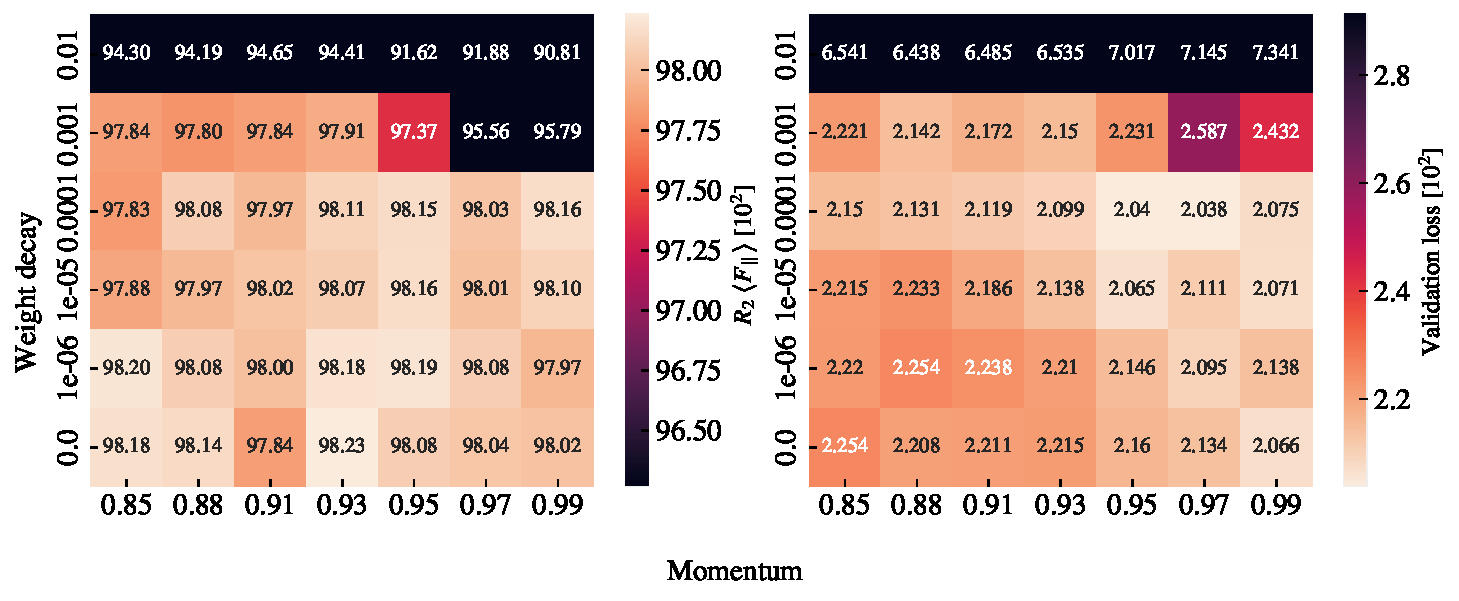
\includegraphics[width=0.8\textwidth]{figures/ML/mom_weight_search_constant_perf.pdf}
      \caption{Validation performance.}
      % \label{fig:}
  \end{subfigure}
  \hfill
  \begin{subfigure}[t]{\textwidth}
      \centering
      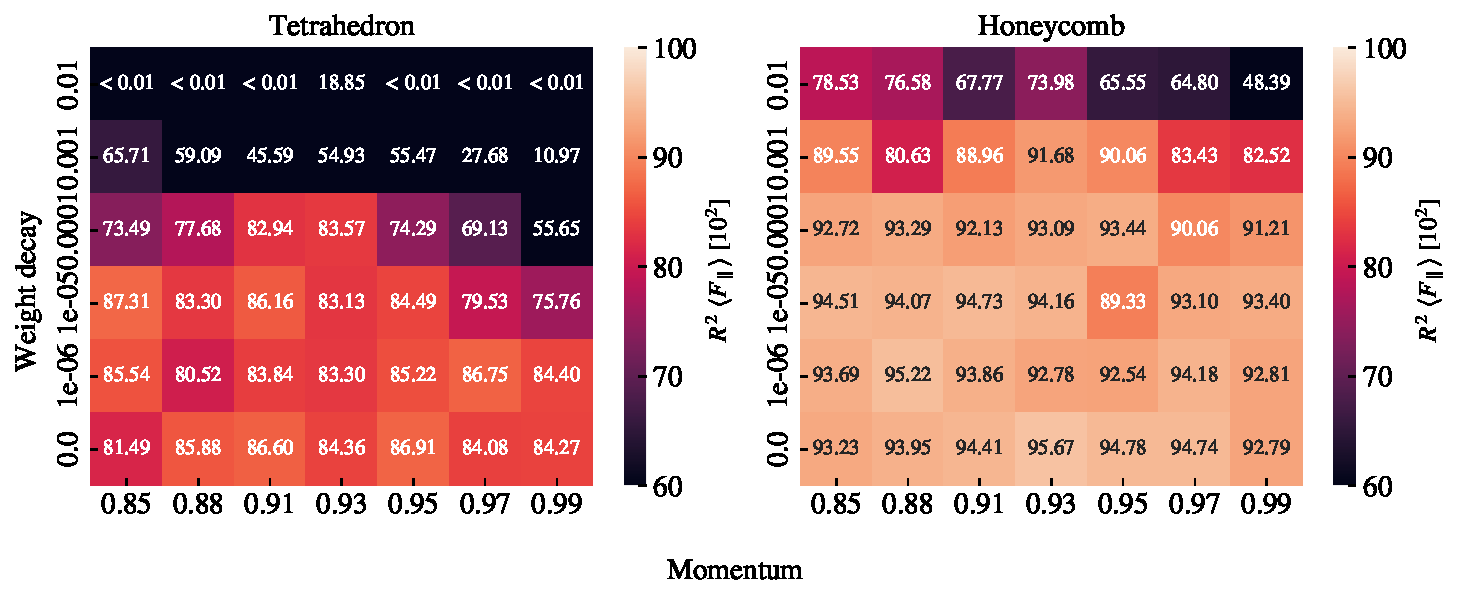
\includegraphics[width=0.8\textwidth]{figures/ML/mom_weight_search_compare_constant_perf.pdf}
      \caption{Selected set comparison.}
      % \label{fig:}
  \end{subfigure}
  \hfill
  \caption{Momentum and weight decay grid search using a constant learning rate corresponding to the results from the learning rate range test in~\cref{fig:LR_range_mom}. (a) The friction mean $R^2$ validation score (left) and the validation loss (right). (b) The friction mean $R^2$ validation score for the selected set of Honeycomb (left) and Tetrahedron (right) patterns respectively, similar to that used in~\cref{fig:A_search_compare}.}
  \label{fig:mom_weight_search_constant}
\end{figure}

\begin{figure}[H]
  \centering
  \begin{subfigure}[t]{1.0\textwidth}
      \centering
      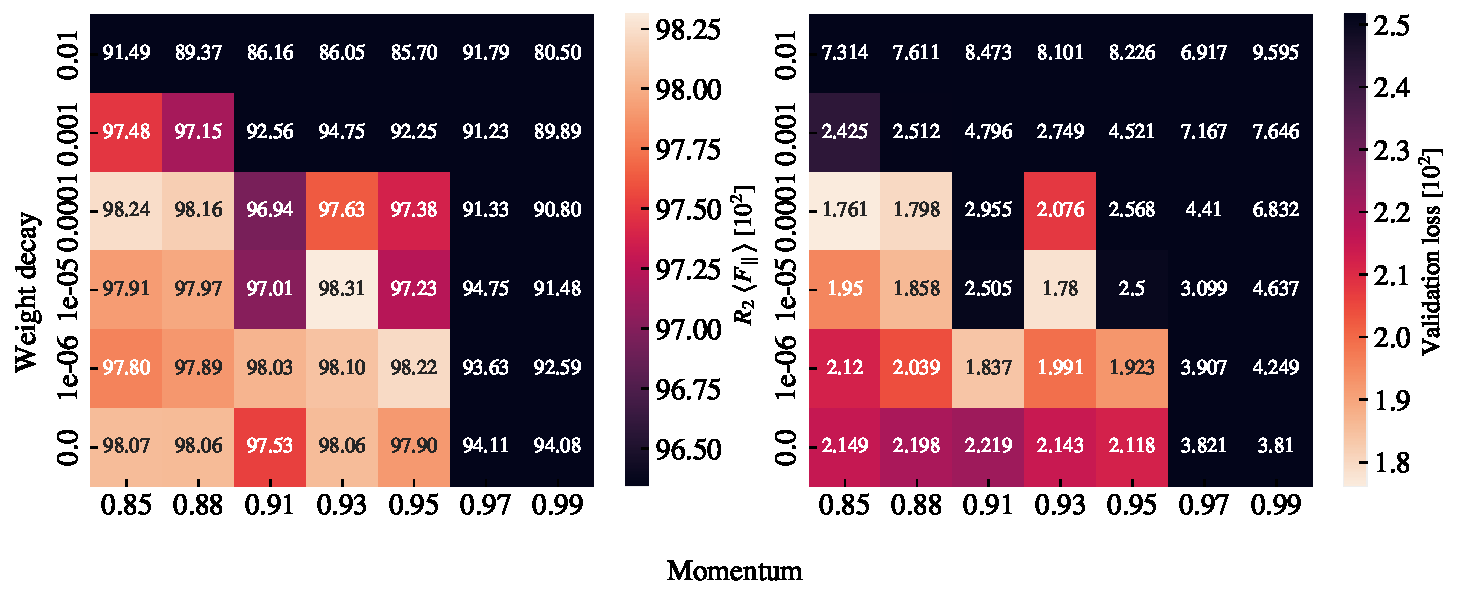
\includegraphics[width=0.8\textwidth]{figures/ML/mom_weight_search_cyclic_perf.pdf}
      \caption{Validation performance.}
      % \label{fig:}
  \end{subfigure}
  \hfill
  \begin{subfigure}[t]{1.0\textwidth}
      \centering
      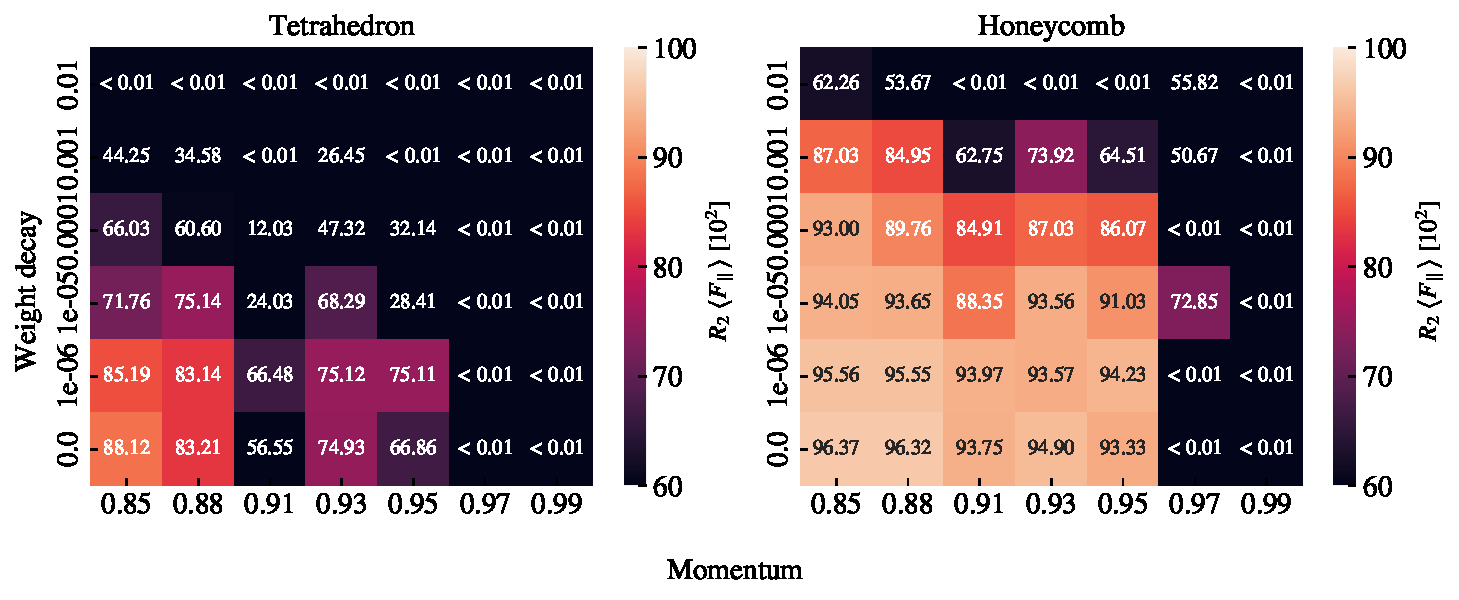
\includegraphics[width=0.8\textwidth]{figures/ML/mom_weight_search_compare_cyclic_perf.pdf}
      \caption{Selected set comparison.}
      % \label{fig:}
  \end{subfigure}
  \hfill
  \caption{Momentum and weight decay grid search using a cyclic learning rate and cyclic momentum scheme. The learning rate maximum bound is chosen according to the learning rate range test in~\cref{fig:LR_range_mom}. The learning rate starts from a factor $1/20$ of the maximum bound, increases toward the maximum bound during the first $30\%$ of training and decreases toward a factor \num{e-4} of the maximum bound for the remaining 70\% of training. This is done by following a cosine curve. The momentum performs an inverse cycling with the lowest momentum of 0.80 at the highest learning rate and a peak in momentum, corresponding to the values in the grid search, at the lowest learning rate. (a) The friction mean $R^2$ validation score (left) and the validation loss (right). (b) The friction mean $R^2$ validation score for the selected set of Honeycomb (left) and Tetrahedron (right) patterns respectively, similar to that used in~\cref{fig:A_search_compare}.}
  \label{fig:mom_weight_search_cyclic}
\end{figure}

The original validation scores, before varying momentum and weight decay, were a
validation loss of 0.02124 and a mean friction $R^2$ score of 0.9816. By varying
momentum and weight decay, we find that these scores can be improved slightly
for the constant learning rate scheme (loss: 0.02038, $R^2$: 0.9823) and even
more for the cyclic scheme (loss: 0.0176, $R^2$: 0.9831). Note that the loss and
$R^2$ scores here do not correspond to the same hyperparameter choices. The
comparison among best scores is summarized in~\cref{tab:mom_weight_search}. In
general, the constant scheme shows rather stable results for all momentum
settings $m \in [0.85, 0.99]$ in combination with a low weight decay $\lambda
\le \num{e-4}$. For the cyclic scheme the performance peaks toward a low
momentum $m \le 0.93$ and a low weight decay $\lambda \le \num{e-4}$. Looking at
the summary in~\cref{tab:mom_weight_search}, we see that the cyclic scheme can
produce a high score among all four performance metrics, but since these scores
do not share common hyperparameters we need to choose which of them to
prioritize. Due to our interest in capturing the non-linear trends, we
prioritize the score from the selected set of Tetrahedron patterns as this has
proven to be the greatest challenge for our model to capture. We recognize that this
choice introduces a greater risk of overfitting since the data points within
this evaluation set are partly included in the training set as well. This is
especially alarming since the absence of weight decay allows for more
overfitting in general. However, for the purpose of performing an accelerated
search, we find it more important to increase the likelihood of discovering
novel designs than to reduce the risk of getting false positive results. Since
we retain the option to verify the properties of a given design through
\acrshort{MD} simulations afterward, we do not have to rely on the machine
learning prediction indefinitely. Thus we choose the cyclic trained model with
low maximum momentum $m = 0.85$ and zero weight decay as our final model. On a final
note, we also point out that our choice of hyperparameters corresponded to the
edge of our grid search. Thus, it would have been natural to perform an extended
search in that range, but due to time constraints and the belief that the potential gain from doing so was not significant, we decided to omit it.


\begin{table}[!htb]
  \begin{center}
  \caption{The best validation loss and $R^2$ scores from the momentum and weight grid search using the S32D12 model. We compare the scores from the constant and cycling learning rate and momentum scheme against the original scores from the S32D12 model in the architecture complexity grid search. The scores correspond to different hyperparameter choices that maximize each score respectively.}
  \label{tab:mom_weight_search}
  \begin{tabular}{|c|c|c|c|c|} \hline
     &  & Score [\num{e2}] & Momentum & Weight decay \\ \hline
     \multirow{3}{*}{Validation loss} & Original & 2.124 & 0.9 & 0  \\ 
      & Constant & 2.038 & 0.97 & \num{e-4} \\ 
      & Cyclic & 1.761 & 0.85 & \num{e-4} \\ \hline
     \multirow{3}{*}{Validation $R^2$} & Original & 98.16 & 0.9 & 0  \\ 
      & Constant & 98.23 & 0.93 & 0 \\ 
      & Cyclic & 98.31 & 0.93 & \num{e-5} \\ \hline
     \multirow{3}{*}{Tetrahedron $R^2$} & Original & 87.07 & 0.9 & 0  \\ 
      & Constant & 87.31 & 0.85 & \num{e-5} \\ 
      & Cyclic & 88.12 & 0.85 & 0 \\ \hline
     \multirow{3}{*}{Honeycomb $R^2$} & Original & 94.78 & 0.9 & 0  \\ 
      & Constant & 95.67 & 0.93 & 0 \\ 
      & Cyclic & 96.37 & 0.85 & 0 \\ \hline
  \end{tabular}
  \end{center}
\end{table}



\subsection{Model performance}
From the hypertuning process, we settled on the S32D12 model trained by a cyclic scheme with a maximum momentum of 0.85, a maximum learning rate bound of $0.015$ chosen accordingly to the learning range test in~\cref{fig:LR_range_mom} and zero weight decay. The model contains
\num{1.3e7} model parameters. The main performance metrics are shown
in~\cref{tab:final_model_eval} where ``Tetrahedron'' and ``Honeycomb'' refer to
the selected set scores. Although we have mainly considered the mean friction
$R^2$ score during the hypertuning we find that the performance on the remaining
parameters is reasonable as well. The validation set reveals a final $R^2$ score
for the mean friction of $\sim 98 \%$ and a rupture accuracy of $\sim 96 \%$.
Since the data only contains roughly $12 \%$ ruptures this should be compared to
a score of $88 \%$ corresponding to simply predicting no ruptures at all. We find a considerably large relative error for the rupture strain of
$\sim 13 \%$. However, this error is lower for the Tetrahedron ($5.9\%$) and Honeycomb ($1.5\%$) sets. Hence, it is possible to infer that the high relative error in the validation set is due to some instances of very low rupture strains that might shift up the average value for the relative error. \cref{fig:final_model_eval} shows the mean friction, max friction and relative contact predictions for the Tetrahedron $(7, 5, 1)$ and Honeycomb $(2,2,1,5)$ patterns used in the pilot study. We note that these configurations are also partly contained in the training data, but this serves as a way of comparing the prediction quality estimated for the $R^2$ scores with a visual evaluation. Later on, we will evaluate a true test set based on the proposals from the accelerated search. 


\begin{table}[!htb]
  \begin{center}
  \caption{Evaluation of the final model performance considering all the model outputs. Mean values are taken over the scores for each configuration within the categories: The validation set, the selected Tetrahedron set and the selected Honeycomb set.}
  \label{tab:final_model_eval}
  \begin{tabular}{ | c | c | c | c | c | c | c | c |} \hline
    & Loss [\num{e2}] & \multicolumn{3}{c|}{$R^2$ [\num{e2}]} & Abs. [\num{e2}] & Rel. [\num{e2}]  & Acc. [\num{e2}] \\ \hline
    & Total & Mean $F_f$ & Max $F_f$ & Contact & Porosity & Rup.\ Strain & Rupture \\ \hline
  Validation  & 2.1488 & 98.067 & 93.558 & 94.598 & 2.325 & 12.958 & 96.102 \\ \hline
  Tetrahedron & 4.0328 & 88.662 & 85.836 & 64.683 & 1.207 & \phantom{0}5.880 & 99.762 \\ \hline
  Honeycomb   & 8.6867 & 96.627 & 89.696 & 97.171 & 1.040 & \phantom{0}1.483 & 99.111 \\ \hline
  \end{tabular}
  \end{center}
\end{table}


With the use of our final model, we evaluate the performance for the task of
ranking the configurations by the properties of interest. That is, we go through
all the configurations in the dataset, for the Tetrahedron, Honeycomb and Random
walk respectively, calculate the properties of interest and sort the
configurations accordingly. This is shown in~\cref{tab:ML_ranking} in comparison to the actual
ranking in the dataset. Generally, we find that the \acrshort{ML} model performs
rather well in the ranking of the maximum properties getting the right
configurations into the top 3 three, while it is performing a lot worse for the
minimum friction property. This latter observation can be
attributed to the fact that the precision needed for an accurate ranking among
the minimum friction cases is a lot higher than for the remaining properties. This lack of precision is especially highlighted by the fact that the model predicts the $12\text{th}$ Random walk pattern (see~\cref{tab:ML_ranking_RW}) to have negative mean friction, which is clearly outside the bound of reasonable values. For the maximum categories, we find that the model gives a slightly
better ranking for the Tetrahedon and Honeycomb in comparison to the Random walk
patterns. When considering the actual predicted property scores for the maximum
properties we find that the model predictions are generally within a $\sim 0.2$
nN deviation in the top 5. This supports that our model can be used to perform
an accelerated search of new configurations yielding a meaningful ranking of
property scores. 


\begin{figure}[H]
  \centering
  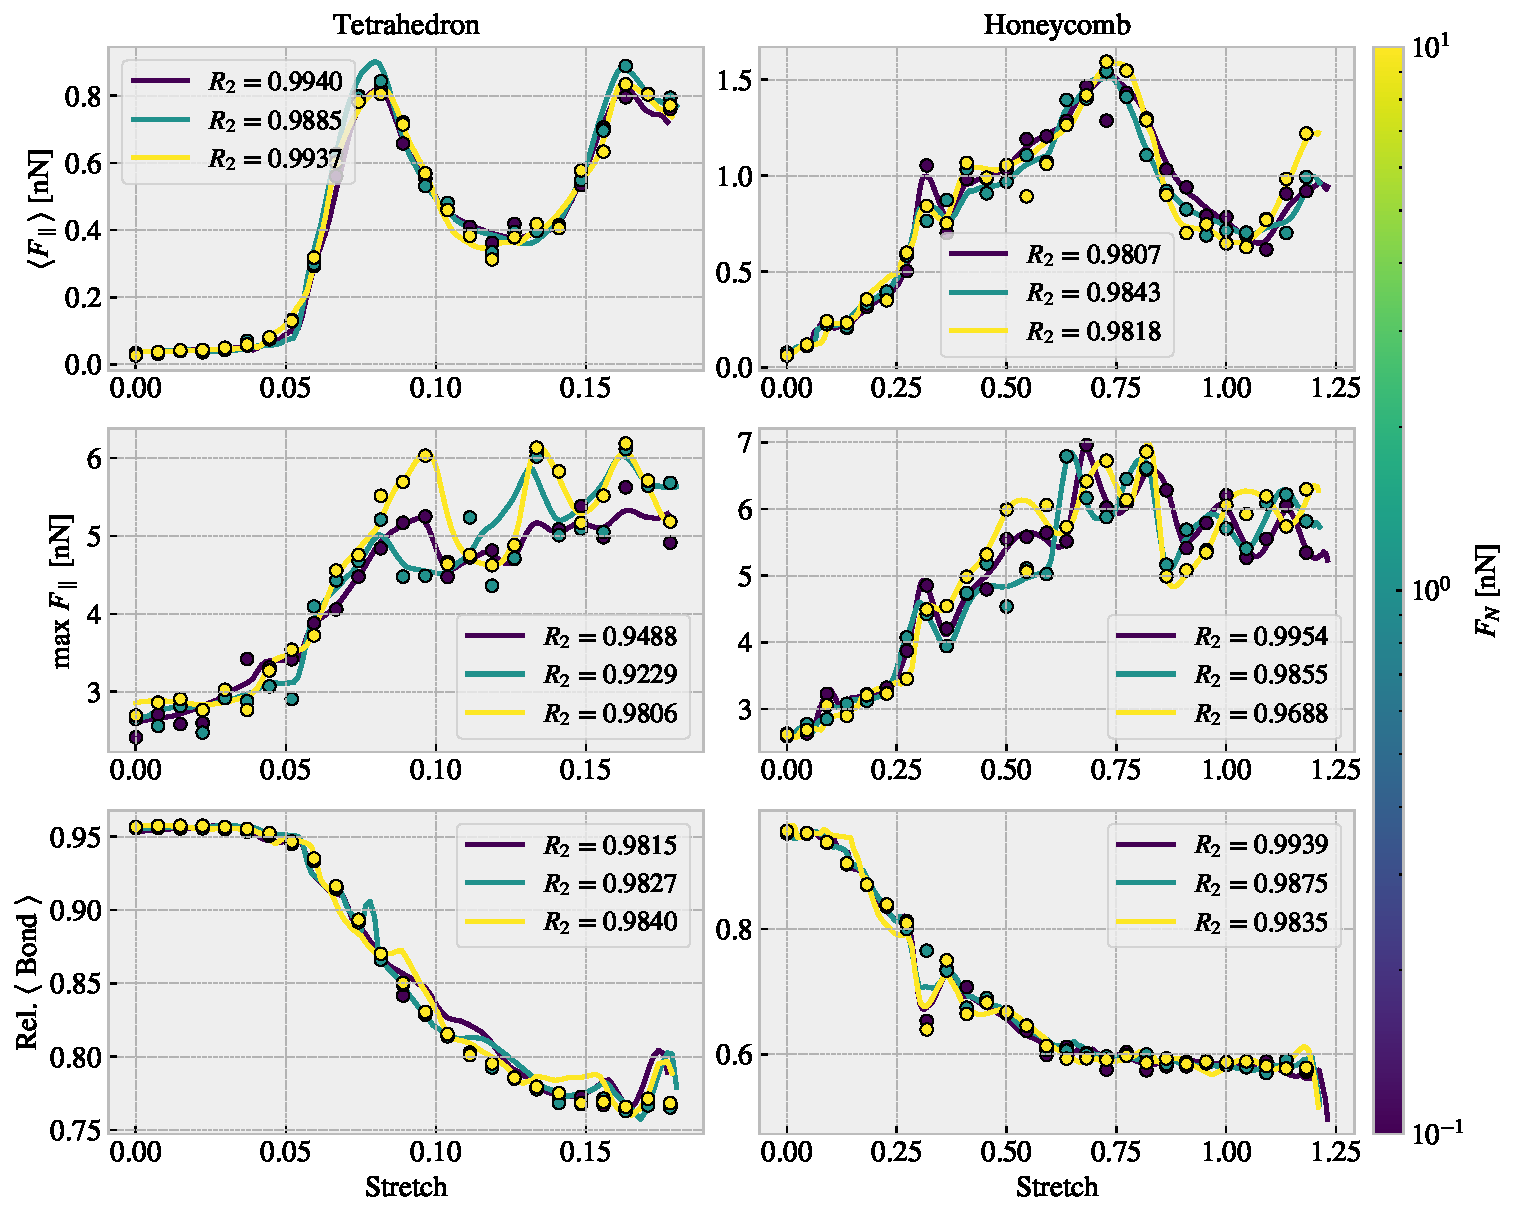
\includegraphics[width=\linewidth]{figures/ML/final_model_evaluation.pdf}
  \caption{Visual evaluation of the final model predictions on the Tetrahedron $(7,5,1)$ and Honeycomb $(2,2,1,5)$ used in the pilot study, for the mean friction $\langle F_{\parallel} \rangle$, maximum friction $\max F_\parallel$ and the relative contact as a function of strain. The model predictions (solid line) are based on \num{e3} data points in the strain range [0, 1.5], with the curve being cut off after the first rupture prediction. This is compared to the data points (dots). The color denotes the corresponding normal loads. The $R^2$ scores are shown for each prediction fit for each load value.}
  \label{fig:final_model_eval}
\end{figure}  



\begin{table}[H]
  \begin{subtable}[t]{1\textwidth}
    \centering
    \begin{tabular}{|c|C{2cm}|c?{0.3mm}C{2cm}|c|c|} \hline
      ML & \multicolumn{2}{c?{0.3mm}}{Data} &  \multicolumn{2}{c|}{\acrshort{ML}} & Data \\ \cline{2-5}
      Rank & Config & Value [nN] & Config & Value [nN] & Rank \\ \hline
      \multicolumn{6}{|c|}{$\min F_{\text{fric}}$} \\ \hline
      20 & (3, 9, 4) & 0.0067 & (3, 1, 2) & 0.0041 & 5  \\ \hline
      5 & (3, 1, 3) & 0.0075 & (1, 3, 4) & 0.0049 & 11 \\ \hline
      6 & (5, 3, 4) & 0.0084 & (1, 3, 3) & 0.0066 & 6  \\ \hline
      21 & (1, 7, 3) & 0.0084 & (3, 1, 4) & 0.0066 & 8  \\ \hline
      1 & (3, 1, 2) & 0.0097 & (3, 1, 3) & 0.0078 & 2  \\ \hline
      \multicolumn{6}{|c|}{$\max F_{\text{fric}}$} \\ \hline
      1 & (5, 3, 1) & 1.5875 & (5, 3, 1) & 1.5920 & 1 \\ \hline
      2 & (1, 3, 1) & 1.4310 & (1, 3, 1) & 1.2739 & 2 \\ \hline
      4 & (3, 1, 2) & 1.0988 & (9, 3, 1) & 1.1162 & 4 \\ \hline
      3 & (9, 3, 1) & 1.0936 & (3, 1, 2) & 0.7819 & 3 \\ \hline
      5 & (7, 5, 1) & 0.7916 & (7, 5, 1) & 0.7740 & 5 \\ \hline
      \multicolumn{6}{|c|}{$\max \Delta F_{\text{fric}}$} \\ \hline
      1 & (5, 3, 1) & 1.5529 & (5, 3, 1) & 1.5578 & 1 \\ \hline 
      2 & (1, 3, 1) & 1.3916 & (1, 3, 1) & 1.2331 & 2 \\ \hline 
      4 & (3, 1, 2) & 1.0891 & (9, 3, 1) & 1.0807 & 4 \\ \hline 
      3 & (9, 3, 1) & 1.0606 & (3, 1, 2) & 0.7778 & 3 \\ \hline 
      5 & (7, 5, 1) & 0.7536 & (7, 5, 1) & 0.7399 & 5 \\ \hline 
      \multicolumn{6}{|c|}{max drop} \\ \hline
      1 & (5, 3, 1) & 0.8841 & (5, 3, 1) & 0.8603 & 1 \\ \hline 
      2 & (3, 5, 1) & 0.4091 & (3, 5, 1) & 0.3722 & 2 \\ \hline 
      4 & (7, 5, 1) & 0.3775 & (1, 1, 1) & 0.2879 & 5 \\ \hline 
      5 & (9, 7, 1) & 0.2238 & (7, 5, 1) & 0.2478 & 3 \\ \hline 
      3 & (1, 1, 1) & 0.1347 & (9, 7, 1) & 0.1302 & 4 \\ \hline 
    \end{tabular}
  \caption{Tetrahedron ranking. }
  \label{tab:ML_ranking_pop}
  \end{subtable}
  \vspace{5mm}
  \newline
  \begin{subtable}[t]{1\textwidth}
  \centering
  \begin{tabular}{|c|C{2cm}|c?{0.3mm}C{2cm}|c|c|} \hline
    ML & \multicolumn{2}{c?{0.3mm}}{Data} &  \multicolumn{2}{c|}{\acrshort{ML}} & Data \\ \cline{2-5}
    Rank & Config & Value [nN] & Config & Value [nN] & Rank \\ \hline
    \multicolumn{6}{|c|}{$\min F_{\text{fric}}$} \\ \hline
    1 & (2, 5, 1, 1) & 0.0177 & (2, 5, 1, 1) & 0.0113 & 1 \\ \hline 
    9 & (2, 4, 5, 1) & 0.0187 & (2, 5, 5, 3) & 0.0149 & 7 \\ \hline 
    7 & (2, 4, 1, 1) & 0.0212 & (2, 5, 5, 1) & 0.0182 & 4 \\ \hline 
    3 & (2, 5, 5, 1) & 0.0212 & (2, 5, 3, 1) & 0.0186 & 5 \\ \hline 
    4 & (2, 5, 3, 1) & 0.0226 & (2, 4, 1, 3) & 0.0198  & 15 \\ \hline 
    \multicolumn{6}{|c|}{$\max F_{\text{fric}}$} \\ \hline
    1 & (2, 1, 1, 1) & 2.8903 & (2, 1, 1, 1) & 2.9171 & 1 \\ \hline 
    2 & (2, 1, 5, 3) & 2.2824 & (2, 1, 5, 3) & 2.4004 & 2 \\ \hline 
    6 & (2, 1, 3, 1) & 2.0818 & (2, 1, 5, 1) & 2.1060 & 5 \\ \hline 
    4 & (2, 1, 3, 3) & 2.0313 & (2, 1, 3, 3) & 1.9458 & 4 \\ \hline 
    3 & (2, 1, 5, 1) & 2.0164 & (2, 4, 1, 1) & 1.9381 & 6 \\ \hline 
    \multicolumn{6}{|c|}{$\max \Delta F_{\text{fric}}$} \\ \hline
    1 & (2, 1, 5, 3) & 2.0234 & (2, 1, 5, 3) & 2.1675 & 1 \\ \hline 
    2 & (2, 1, 1, 1) & 1.9528 & (2, 1, 1, 1) & 2.0809 & 2 \\ \hline 
    3 & (2, 4, 1, 1) & 1.8184 & (2, 4, 1, 1) & 1.9157 & 3 \\ \hline 
    4 & (2, 1, 3, 3) & 1.7645 & (2, 1, 3, 3) & 1.6968 & 4 \\ \hline 
    5 & (2, 4, 1, 3) & 1.4614 & (2, 4, 1, 3) & 1.5612 & 5 \\ \hline 
    \multicolumn{6}{|c|}{max drop} \\ \hline
    1 & (2, 3, 3, 3) & 1.2785 & (2, 3, 3, 3) & 1.3642 & 1 \\ \hline 
    2 & (2, 1, 3, 1) & 1.1046 & (2, 1, 3, 1) & 0.9837 & 2 \\ \hline 
    3 & (2, 3, 3, 5) & 0.8947 & (2, 3, 3, 5) & 0.9803 & 3 \\ \hline 
    4 & (2, 1, 5, 3) & 0.8638 & (2, 1, 5, 3) & 0.9556 & 4 \\ \hline 
    13 & (2, 5, 1, 1) & 0.8468 & (2, 4, 5, 3) & 0.8999 & 8 \\ \hline 
  \end{tabular}
  \caption{Honeycomb ranking.}
  \label{tab:ML_ranking_hon}
  \end{subtable}  
  \caption{(Table continues on the next page)}
  \end{table}

\begin{table}[H]\ContinuedFloat
  \begin{subtable}[t]{1\textwidth}
  \centering
  \begin{tabular}{|c|C{2cm}|c?{0.3mm}C{2cm}|c|c|} \hline
    ML & \multicolumn{2}{c?{0.3mm}}{Data} &  \multicolumn{2}{c|}{\acrshort{ML}} & Data \\ \cline{2-5}
    Rank & Config & Value [nN] & Config & Value [nN] & Rank \\ \hline
    \multicolumn{6}{|c|}{$\min F_{\text{fric}}$} \\ \hline
    1 & 12 & 0.0024 & 12 & $-0.0011 \ $ & 1 \\ \hline 
    24 & 76 & 0.0040 & 06 & 0.0036  & 27 \\ \hline 
    6 & 13 & 0.0055 & 14 & 0.0074  & 23 \\ \hline 
    31 & 08 & 0.0065 & 05 & 0.0082  & 19 \\ \hline 
    26 & 07 & 0.0069 & 63 & 0.0085  & 57 \\ \hline 
    \multicolumn{6}{|c|}{$\max F_{\text{fric}}$} \\ \hline
    3 & 96 & 0.5758 & 99 & 0.5155 & 2 \\ \hline 
    1 & 99 & 0.5316 & 98 & 0.4708 & 3 \\ \hline 
    2 & 98 & 0.4478 & 96 & 0.4356 & 1 \\ \hline 
    4 & 97 & 0.3624 & 97 & 0.3503 & 4 \\ \hline 
    11 & 58 & 0.3410 & 55 & 0.2817 & 7 \\ \hline 
    \multicolumn{6}{|c|}{$\max \Delta F_{\text{fric}}$} \\ \hline
    3 & 96 & 0.5448 & 99 & 0.4669 & 2 \\ \hline 
    1 & 99 & 0.4769 & 98 & 0.4314 & 3 \\ \hline 
    2 & 98 & 0.4085 & 96 & 0.4128 & 1 \\ \hline 
    4 & 97 & 0.3268 & 97 & 0.3080 & 4 \\ \hline 
    78 & 57 & 0.2978 & 55 & 0.2542 & 7 \\ \hline 
    \multicolumn{6}{|c|}{max drop} \\ \hline
    3 & 01 & 0.1818 & 00 & 0.1883 & 3 \\ \hline 
    2 & 96 & 0.1733 & 96 & 0.1654 & 2 \\ \hline 
    1 & 00 & 0.1590 & 01 & 0.1532 & 1 \\ \hline 
    11 & 37 & 0.1022 & 04 & 0.0591 & 8 \\ \hline 
    28 & 34 & 0.0879 & 56 & 0.0552 & 20 \\ \hline 
  \end{tabular}
  \caption{Random walk ranking.}
  \label{tab:ML_ranking_RW}
  \end{subtable}  
  \caption{Ranking of the dataset according to the four properties of interest using the final machine learning (\acrshort{ML}) model for the Tetrahedon (a), Honeycomb (b) and Random walk (c) patterns in the dataset respectively. The ranking is shown in descending order for each section of rows corresponding to the four properties of interest. The left side of the vertical center line denotes the true data ranking showing the top 5 scores in descending order (the top row shows rank 1 and the bottom row shows rank 5). The outermost left column (\acrshort{ML} rank) then denotes the corresponding ranks given by the \acrshort{ML} model. The right side of the vertical center line shows the top 5 ranking given by the \acrshort{ML} model for which the outermost right column shows the corresponding true data ranks. If the model gets the top 5 ranking right both the outermost left and right columns show $1,2,3,4,5$ in descending order.}
  \label{tab:ML_ranking}
  \end{table}




\section{Accelerated Search}
From~\cref{eq:ML} we have found promising results that we can use our machine learning model to predict the frictional behavior of a Kirigami sheet. This enables us to omit the \acrshort{MD} simulations in the evaluation process and perform an accelerated search through new configurations. We will use the friction properties of interest as our main metrics for optimization. We approach the accelerated search by two different methods:
\begin{enumerate}
  \item Using the generative algorithms developed for the creation of the Tetrahedron, Honeycomb and Random walk patterns, we create an extended dataset and evaluate the performance using the \acrshort{ML} model.
  \item Using a genetic algorithm method we perturb (mutate) the configurations and optimize for the max drop property using the \acrshort{ML} model to evaluate the fitness function. 
\end{enumerate}

\subsection{Patteren generation search}\label{sec:gen_search}
We utilize the pattern generators developed in~\cref{chap:system} to create an
extended dataset for our search. For the Tetrahedron and Honeycomb patterns, the
increments of the parameters will eventually lead to the main pattern structures
exceeding the size of the sheet. Thus, we can essentially perform a full search
``maxing out'' the parameters of these patterns. We estimate that this is done
with the maximum parameters, $(60, 60, 30)$ for the Tetrahedron, and $(30, 30, 30,
60)$ for the Honeycomb pattern. We use a random reference position and
regenerate each unique parameter set 10 times to explore translational effects. This
gives in total \num{1.35e5} configurations for the Tetrahedron pattern and
\num{2.025e6} for the Honeycomb pattern. For the Random walk generator, we perform a
Monte Carlo sampling. That is, in each sample we draw the scalar values, either from a
uniform (U) or logarithmic uniform (LU) distribution as follows.
\begin{align*}
  \text{Num.\ walks}, & \sim \text{U}[1, 30], & \text{Max.\ steps}, &\sim \text{U}[1,30], & \text{Min.\ dis.}, & \sim \text{U}[0,4], \\
  \text{Bias direction}, &\sim \text{U}[0, 2\pi], & \text{Bias.\ strength}, &\sim \text{LU}[0,10],  & p_{\text{stay}}, &\sim \text{U}[0,1].
\end{align*}
Notice that we use a discrete distribution for the parameters requiring
integers. For the binary parameters \textit{connection}, \textit{avoid invalid},
\textit{RN6} and \textit{grid start} we simply set the values by a 50--50
chance. The remaining parameters are kept constant at \textit{periodic} set to
true and \textit{centering} set to false throughout the search. For the handling
of clustering, we implement the extended repair algorithm such that the sheet is repaired by the least modifications approach rather than retrying the generation several times. Due to the extra
computation time associated with the random walk and the repair algorithm, we
only generate \num{e4} configurations within this class. For the \acrshort{ML}
evaluation of the generated configurations we use a normal load of \SI{5}{nN} and generate
a friction-strain curve in the strain domain $[0,2]$ using 100 uniformly spaced points. We compute
the properties of interest and rank the configurations accordingly. The top
candidate scores for each property are shown in~\cref{tab:pattern_search} including a comparison to the original dataset top candidates (from~\cref{tab:data_properties}). The random walk top five candidates for each property respectively are visualized in~\cref{fig:RW_search_top5}.


\begin{table}[!htb]
  \begin{center}
  \caption{Results for the accelerated search using the pattern generators. The top search candidates for each of the four properties of interest are shown in the left section (Search) regarding the Tetrahedron, Honeycomb and Random walk patterns respectively. The upper rows show the scores and the lower rows the associated names (parameters). The right section (Data) shows the corresponding scores from the best candidates within the dataset (from~\cref{tab:data_properties}). All scores are given in units nN.}
  \label{tab:pattern_search}
  \begin{tabular}{|L{1.75cm} |c|c|c| c |c|c|c|} \cline{2-4} \cline{6-8}
  \multicolumn{1}{c|}{} & \multicolumn{3}{c|}{Search}  && \multicolumn{3}{c|}{Data} \\ \cline{2-4} \cline{6-8}
  \multicolumn{1}{c|}{\textbf{Scores}} & Tetrahedron & Honeycomb & Random walk && Tetrahedron & Honeycomb & Random walk \\ \cline{1-4} \cline{6-8}
  $\min F_{\text{fric}}$         & $-0.062 \ \ $  & $-0.109 \ \ $  & $-0.061 \ \ $ &&   0.0067 & 0.0177 & 0.0024 \\ \cline{1-4} \cline{6-8}
  $\max F_{\text{fric}}$         & $1.089$        & $2.917$        & $0.660$       &&   1.5875 & 2.8903 & 0.5758 \\ \cline{1-4} \cline{6-8}
  $\max \Delta F_{\text{fric}}$  & $1.062$        & $2.081$        & $0.629$       &&   1.5529 & 2.0234 & 0.5448 \\ \cline{1-4} \cline{6-8}   
  max drop                      & $0.277$        & $1.250$        & $0.269$       &&   0.8841 & 1.2785 & 0.1818 \\ \cline{1-4} \cline{6-8}   
  \multicolumn{8}{c|}{} \\ \cline{2-4} \cline{6-8}
  \multicolumn{1}{c|}{\textbf{Configs.}} & Tetrahedron & Honeycomb & Random walk  && Tetrahedron & Honeycomb & Random walk  \\ \cline{1-4} \cline{6-8}
  $\min F_{\text{fric}}$         & $(13,11,14)$ & $(14,25,7,19)$  & \textit{no name} &&   $(3,9,4)$ & $(2,5,1,1)$ & 12 \\ \cline{1-4} \cline{6-8}
  $\max F_{\text{fric}}$         & $(1,3,1)$    & $(2,1,1,1)$     & \textit{no name} &&   $(5,3,1)$ & $(2,1,1,1)$ & 96 \\ \cline{1-4} \cline{6-8}
  $\max \Delta F_{\text{fric}}$  & $(1,3,1)$    & $(2,1,1,1)$     & \textit{no name} &&   $(5,3,1)$ & $(2,1,5,3)$ & 96 \\ \cline{1-4} \cline{6-8}   
  max drop                      & $(1,7,1)$    & $(3,3,5,3)$     & \textit{no name} &&   $(5,3,1)$ & $(2,3,3,3)$ & 01 \\ \cline{1-4} \cline{6-8}   
  \end{tabular}
  \end{center}
\end{table}

First of all, we notice that the top candidates for the minimum friction are all
predicted to have a negative friction value. This unphysical prediction aligns
with the previous observations that our model does not have the required
precision to yield accurate predictions for this property. Moreover, we can
argue that pursuing the optimization for a low friction value will eventually
exploit the weaknesses of the model as we reward an unphysical negative value.
In order to resolve this problem it may be necessary to extend the training
dataset and possibly include a physical constraint for positive friction values.
However, by consulting the proposed minimum candidates we find that they all
share the same feature of being sparsely cut. For the Random walk, we see this
visually in~\cref{fig:RW_search_top5}, while for the Tetrahedon and Honeycomb
patterns, this is evident from the configuration parameters shown
in~\cref{tab:pattern_search} where the parameters reveal a high spacing between
the cuts. The porosity of the minimum friction top candidates are all rather low
being $1.5\%$, $5.6\%$, and $1.6\%$ for the Tetrahedron, Honeycomb and Random
walk respectively. This further supports the idea that the Kirigami sheet can
not readily be used to reduce friction (within our system domain) since the
results point toward a non-cut sheet as the best minimum friction candidate.


\begin{figure}[!htb]
  \centering
  \includegraphics[width=\linewidth]{figures/search/RW_search_top5.png}
  \caption{Top 5 candidates for the accelerated search using the Random walk generator. The rows denote the four properties of interest and the columns the top 5 candidates found in the search corresponding to descending scores from left to right. }
  \label{fig:RW_search_top5}
\end{figure}  


Among the remaining maximum properties, we find competing scores with the
Honeycomb and Random walk classes. However, the top-scoring values for the
Honeycomb candidates correspond to configurations already within the original
dataset, which is also the case for the Tetrahedron top candidates. The only
difference is the randomized reference position making for a translated version
of the pattern. When taking a closer look at the full ranking for each property
it becomes apparent that the predictions are highly sensitive to the reference
position parameter used for the Tetrahedron and Honeycomb pattern. Since we repeated the pattern generation 10 times for each parameter set with a random reference position, we initially expected to get a ranking in sets of 10. However, the ranking only
shows contiguous appearing sets in the range of 1--5 which points toward a
dependency on pattern translation. Hence we investigate this further by
evaluating the scores for a systematic change of the reference position. We
generally find the max drop parameter to give the highest variation and thus we
show the max drop scores for the max drop top candidates: Tetrahedron $(1,7,1)$,
$(5,3,1)$ and Honeycomb $(3,3,5,3)$, $(2,3,3,3)$
in~\cref{fig:ref_search_top_data}. The results show that the max drop property prediction varies drastically with the translation of these patterns. The emerging question is
then whether this is grounded in a physical phenomenon or simply a
deficiency in the model. Even though the patterns are periodic in the
x-y-plane, with a period according to the unique number of translations shown in~\cref{fig:ref_search_top_data}, the translation will determine the specific
configuration of the edge. Previous studies of static friction and stick-slip
behavior point to the importance of edge effects~\cite{Varini_2015}, and thus for a sheet where the atoms on the free edge (in the $\pm x$ direction) constitute about 2.5\% of the inner sheet atom count, it is not
unreasonable that the translation might result in a significantly different
outcome. In that case, the search through reference positions highlights that
the translation can be key to optimizing for certain properties. However, the
results might also indicate that the model is either overfitted or that we
simply did not provide enough data to reach a generalization of the complex
physical behavior of the system. The sensible way forward to unravel this would
be to perform additional \acrshort{MD} simulations for translational variants of the same configurations to
investigate for any physical edge dependencies or otherwise strengthen the
model by this data. We leave this suggestion for another study. When considering some of the friction-strain curves corresponding to the result in in~\cref{fig:ref_search_top_data} we also find that the prediction of the rupture point plays an important role in the max drop property score. Since the rupture is often predicted on a descending part of the curve any variation to the rupture strain will affect the max drop property quite significantly.


\begin{figure}[!htb]
  \centering
  \begin{subfigure}[t]{0.49\textwidth}
      \centering
      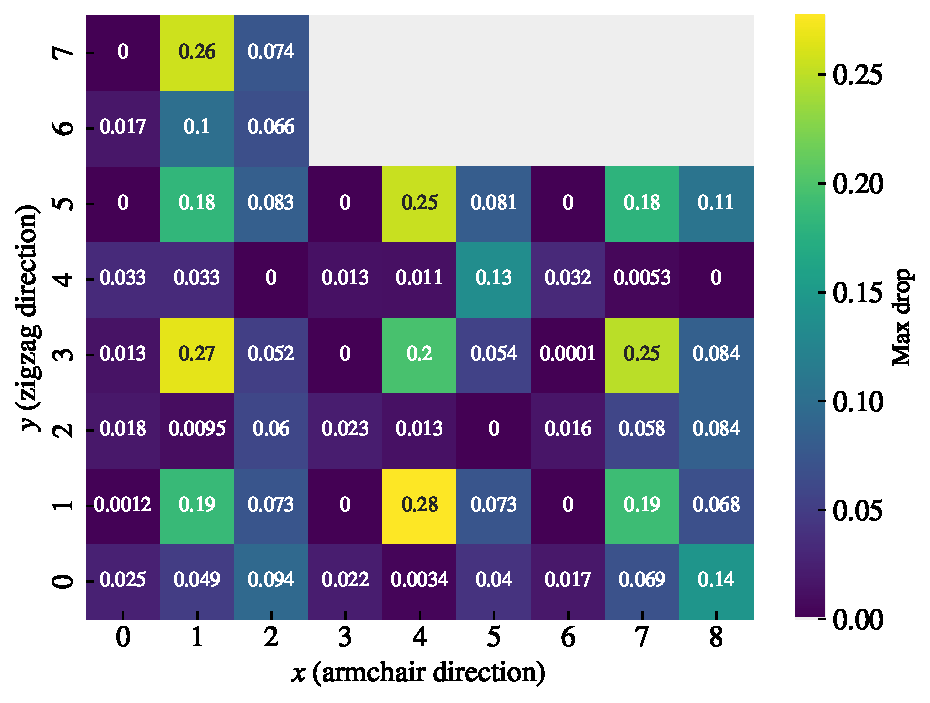
\includegraphics[width=\textwidth]{figures/search/ref_search_drop_pop_1_7_1_ref_search.pdf}
      \caption{Tetrahedron $(1,7,1)$ (60). Std = 0.08, Rel.\ Std = 1.13}
      \label{fig:tetra_171_trans}
  \end{subfigure}
  \hfill
  \begin{subfigure}[t]{0.49\textwidth}
    \centering
    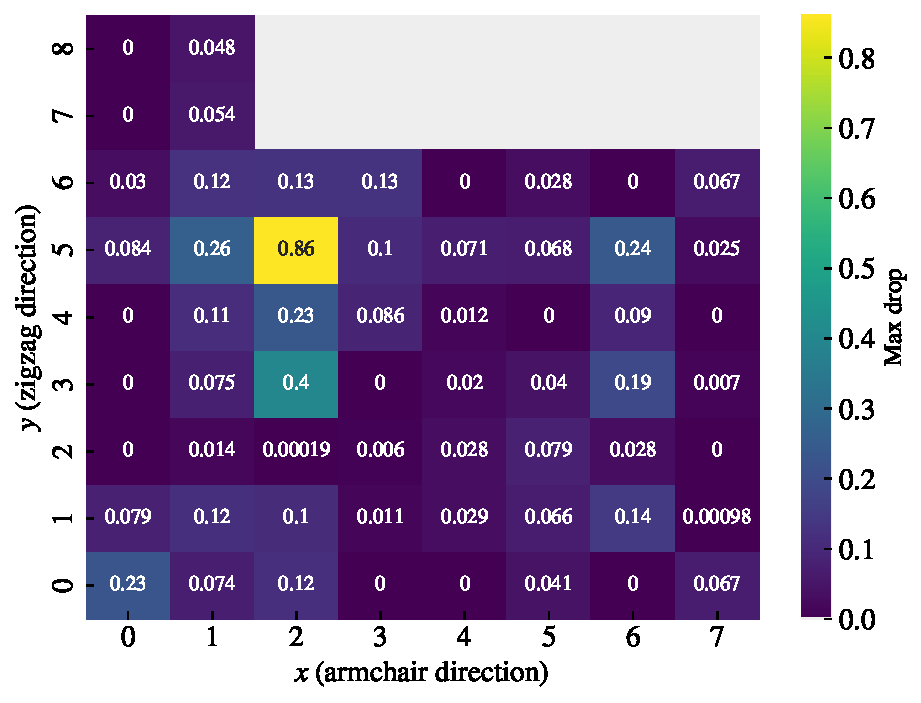
\includegraphics[width=\textwidth]{figures/search/ref_search_drop_pop_5_3_1_ref_search.pdf}
    \caption{Tetrahedron $(5,3,1)$ (60). Std = 0.13, Rel.\ Std = 1.61}
    % \label{fig:}
  \end{subfigure}
  \hfill
  \begin{subfigure}[t]{0.49\textwidth}
      \centering
      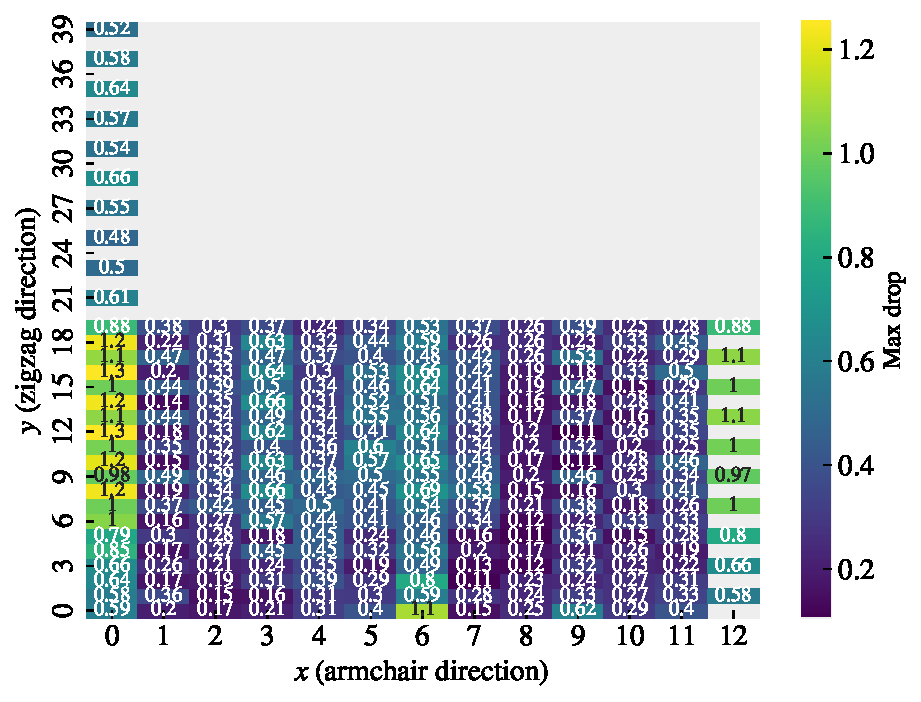
\includegraphics[width=\textwidth]{figures/search/ref_search_drop_hon_3_3_5_3_ref_search.pdf}
      \caption{Honeycomb $(3,3,5,3)$ (260). Std = 0.25, Rel.\ Std = 0.58}
      \label{fig:hon_3353_trans}
      % \label{fig:}
  \end{subfigure}
  \hfill
  \begin{subfigure}[t]{0.49\textwidth}
      \centering
      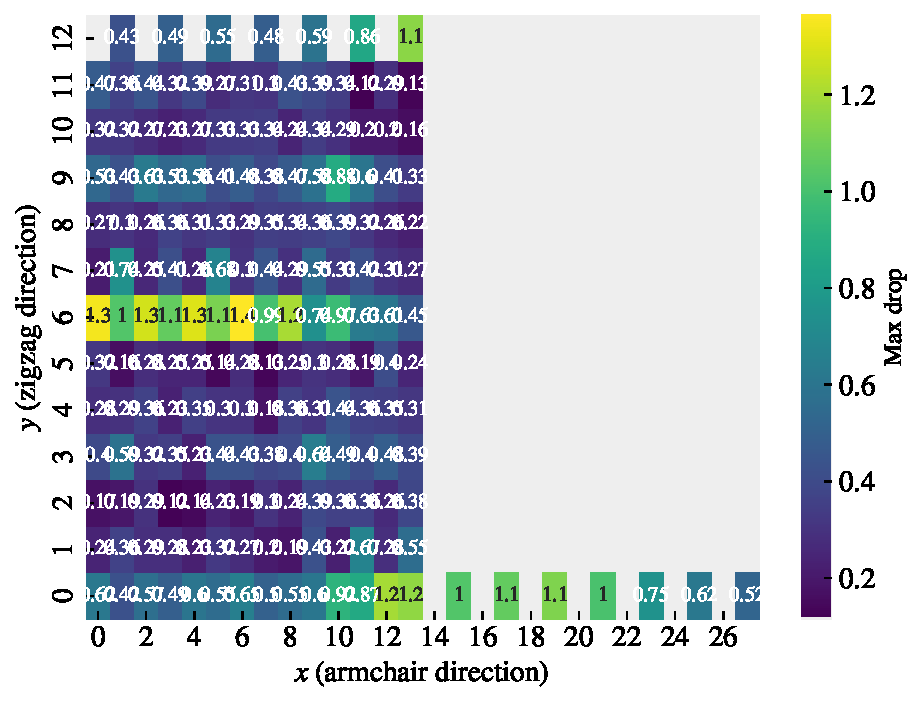
\includegraphics[width=\textwidth]{figures/search/ref_search_drop_hon_2_3_3_3_ref_search.pdf}
      \caption{Honeycomb $(2,3,3,3)$. (182)  Std = 0.27, Rel.\ Std = 0.60}
      % \label{fig:}
  \end{subfigure}
  \hfill
  \caption{Prediction of the max drop property for selected patterns using the machine learning model for all unique reference positions. The heatmap and the annotated values denote the property score with respect to the reference position $x$ and $y$ coordinate. Panels (a) to (d) show the results from various patterns which correspond to the candidates for the max drop property in the accelerated pattern search and the dataset respectively. The sub-caption states the pattern parameters, the number of total unique reference positions in parenthesis, the standard deviation and the standard deviation relative to the mean score. }
  \label{fig:ref_search_top_data}
\end{figure}


In order to get more insight into the generalization of the model, we evaluate
the performance on a true test set. We use the 20 configurations given by the
top 5 Random walk candidates for each of the properties of interest shown in~\cref{fig:RW_search_top5}. We calculate the ground truth data using \acrshort{MD}
simulations with 30 strain values uniformly spaced within the rupture
strain and a normal load of \SI{5}{nN}. Unfortunately, the test
set reveals a substantially worse performance than the validation scores
reported so far. It shows a loss of 2.13, which is two orders of magnitude
higher than the validation loss, an average absolute error for the mean
friction of \SI{0.14}{nN} and a rupture accuracy of 70 \%. The corresponding
mean friction average $R^2$ score is negative which indicates that our model
performs worse than simply guessing on the true data mean. This reveals that our
model is not generalized enough to provide accurate predictions on the newly
generated Random walk configurations. This can mainly be attributed to two
reasons: 1) The test set data distribution is not similar to that of the
training and validation data drawn from the original data set. 2) The
considerations of the selected Tetrahedron and Honeycomb dataset, which
overlapped with the training data, has led to an overfitting of the model in the
hypertuning. In order to test the last hypothesis we went back to the beginning
of the hypertuning process and chose the best model (C16D8) based purely on
validation loss in the architecture complexity grid
test in~\cref{fig:A_search_perf}. By using this model on the test set we find
similar poor results which suggests that the test performance issue is not
caused by the hypertuning process. Instead, it points to the fact that our
original training data does not contain a generalized enough configuration distribution to accurately capture the full complexity of our system. This aligns with the high
fluctuation in prediction value when translating the patterns. Thus we conclude
that a machine learning approach might be feasible, given the promising
validation scores, but that we need a bigger and more generalized dataset for a
reliable prediction of new configurations. 



\subsection{Genetic algorithm search}
Although our machine learning analysis indicates that the model is not generalized enough for an accurate prediction on new configurations, we carry out a short investigation on the use of a genetic-algorithm-based accelerated search. So far we have concluded that a minimization of the friction is not
promising, and hence we discard this property for further study. We have also
seen that the maximum style properties often share similar top candidates, and
thus we choose to only investigate the max drop property associated with the
aim of achieving a negative friction coefficient in the coupled system. 

In order to verify our implementation of the genetic algorithm described
in~\cref{sec:GA}, we consider a smaller $10 \times 10$ square lattice initially. We choose to
evaluate the energy of a zero-temperature Ising model without any external
field. That is, we consider the system described by the Hamiltonian 
\begin{align}
  H = -J\sum_{\langle kl \rangle} s_k s_l,
  \label{eq:H_ising}
\end{align}
where $s$ denotes the value of each lattice site and the sum is running over all
nearest neighbor pairs in the lattice. The sites take a binary value, either
$-1$ or $+1$, meaning that the lowest energy ($-200$) is reached when all site values have an equal sign, all $-1$ or all $+1$. The highest energy ($200$) corresponds to a checkerboard pattern where each site has nearest neighbors with an opposite sign to its own. We consider periodic boundary conditions, meaning that the sites on
the edge will be connected to the sites on the opposite edge. We create a small
population of 10 individuals from a random noise initialization where each site
has a probability of $p$ being $-1$ and a probability $p-1$ being $+1$. Hence, the probability
represents the average porosity of the configurations and we choose $p = 0.5$ as an unbiased choice. When
considering the minimization of energy, the algorithm converges relatively fast (within tens of generations) to the best possible score. Thus, we consider the more challenging problem of maximizing energy which requires the configuration to reach the checkerboard pattern. \cref{fig:ising_max_history} shows the score for a maximization of the energy using the genetic algorithm. We observe that the score converges faster initially, but that it eventually reaches the best score at generation 257. This indicates that the algorithm can handle an optimization problem with some level of spatial dependency. However, we note that some initializations were resulting in a saturating convergence, where two unsynchronized checkerboard patterns formed in distinct regions of the lattice. This leads to a local maximum because transitioning from two unsynchronized checkerboard patterns to a single synchronized pattern would necessitate a slight temporary decrease in the score.

\begin{figure}[!htb]
  \centering
  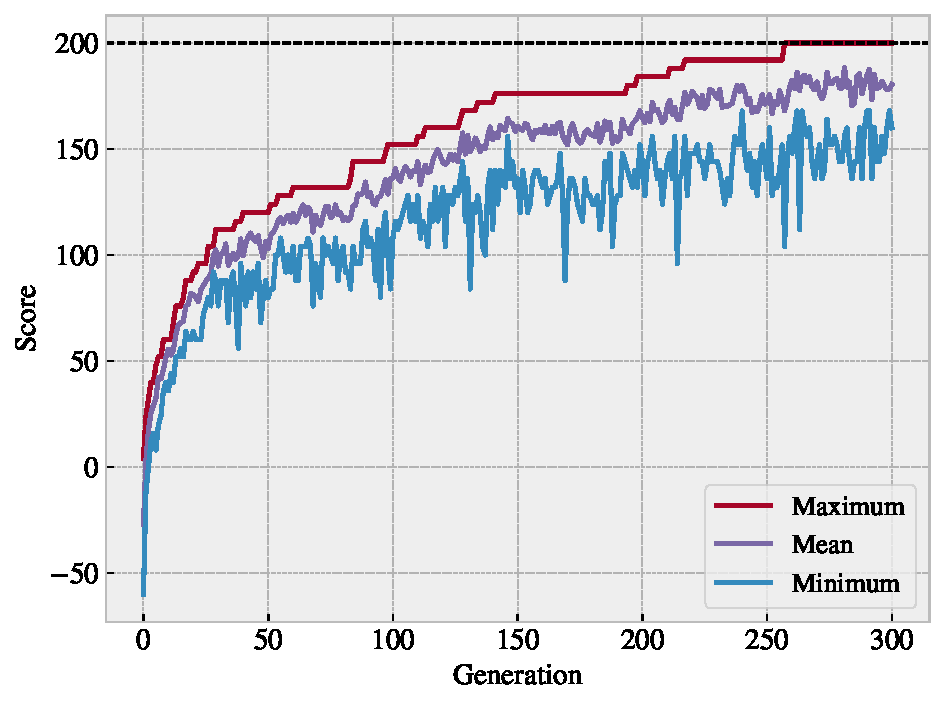
\includegraphics[width=0.6\linewidth]{figures/search/ising_max_history.pdf}
  \caption{Optimization for the maximum Ising energy given by~\cref{eq:H_ising} for a $10 \times 10$ lattice using a population size of 10. The population was initialized with random noise having a probability of 0.5 being $-1$ and a probability of 0.5 being $+1$. The three curves indicate the minimum, mean, and maximum scores in the population. The best score indicated by the dotted line is reached at generation 257. }
  \label{fig:ising_max_history}
\end{figure}  

Moving on from the verification of the algorithm, we consider the optimization
for the max drop property for the Kirigami patterns. We utilize the machine
learning model to evaluate the friction-strain curve for each pattern and
compute the corresponding max drop property value, similar to what we have
done in~\cref{sec:gen_search}. For the initialization of the population, we take
a basis in the top candidates for the pattern generation search
from~\cref{sec:gen_search}. That is, we generate new configurations using the
parameters that led to the highest score for the max drop property. We do this
for the top candidates within the Tetrahedron, Honeycomb and Random walk
categories respectively. We generate a population of 100 configurations and run
the search for 100 generations since we did not see much improvement for longer
runs. 

We find immediately that the Tetrahedron and Honeycomb search did not give any useful results. In both cases, the highest-scoring individual in the population at generation 0 was still the best candidate at the end of the search, even though the average score was rising initially. For the Random walk, we perform 5 runs for different population initializations. We select the top 5 max drop candidates from the Random walk pattern search (seen in the bottom row in~\cref{fig:RW_search_top5}) and use their corresponding parameters for the initializations of the 5 populations. In 4 out of 5 runs, we find a similar result as seen for the Tetrahedon and Honeycomb patterns, meaning that only a single run provided a new pattern for the highest-scoring individual. The score of this individual was \SI{0.240}{nN} which is only a small improvement from the otherwise best Random walk max drop score of
\SI{0.182}{nN}. However, from the other non-improving runs the initialization of the random-walk-based population provided a top score of \SI{0.345}{nN}. This shows that we have better hopes of optimizing the max drop property by simply generating more configurations from these parameters than by running the genetic algorithm. 

Since starting from an existing design did not give any useful results, we attempt to start from a population of random noise as well. We initialize one population with mixed porosities, having 20 individuals each for porosity $\{0.01, 0.05, 0.1, 0.2, 0.3\}$, and two populations based on a constant porosity of 0.25 and 0.5 respectively. This time the algorithm improved the highest-scoring individual throughout, but
the final top scores are still not impressive. The mixed porosity start gave the
highest score, being \SI{0.299}{nN}. When inspecting the top five individuals in the population visually, they were all found rather similar to the starting configurations; they still looked like random noise. Thus, we do not find any significant signs that the genetic algorithm search can contribute with any higher-level pattern structures worth further investigation. We attribute this to the finding that the machine learning model is not reliable for predicting friction for configurations outside the original dataset. However, we acknowledge that the quality of the genetic algorithm results could also be affected by an inadequate number of generations in the search. Nonetheless, given our concerns regarding the machine learning model, we decided not to pursue this any further.

As an attempt to get further insight into the model predictions, we use the Grad-CAM method to examine the top-scoring individuals from the genetic algorithm search. At first, we analyzed the results for each feature map in the network, but we found that taking an average across all feature maps provided a suitable representation of the outcomes. The result for the mixed porosity search is shown in~\cref{fig:GC_mixed_p}. For 
comparison, we included a similar examination for the top candidates in the
pattern generation search, with respect to the max drop category, for the
Tetrahedron, Honeycomb and Random walk, as shown in
\crefrange{fig:GC_pop_search}{fig:GC_RW_search}. For the mixed porosity configuration, the Grad-CAM method highlights some areas in the noise 
as contributing more positively than others, but we do not find any obvious
structure from this. Regarding the Tetrahedron, Honeycomb, and Random Walk configurations with more organized patterns, we observe that the cuts are frequently highlighted. This finding gives some confidence to the notion that the model considers some of the relevant features in the pattern. Nonetheless, the variability of the results is too great to draw any firm conclusions. However, we notice that
for certain strain values, the Grad-CAM reveals considerable ``attention'' toward the edge of the configuration. This especially relates to the top and bottom edge in the $\pm y$ direction. For instance, \cref{fig:GC_hon_search} shows a highlighting of the bottom edge in the friction prediction at a strain of 0.396 for the Honeycomb pattern. Considering that the top and bottom of the configuration are not a true edge, since these are connected to the pull blocks in the simulation, this is a bit surprising. One interpretation is that the dissipation of energy associated with the thermostat in the pull blocks might be of importance. Even though these results should be taken carefully due to the instability of the model, we note this as a topic for further investigation. 


\begin{figure}[!htb]
  \centering
  \begin{subfigure}[t]{1\textwidth}
      \centering
      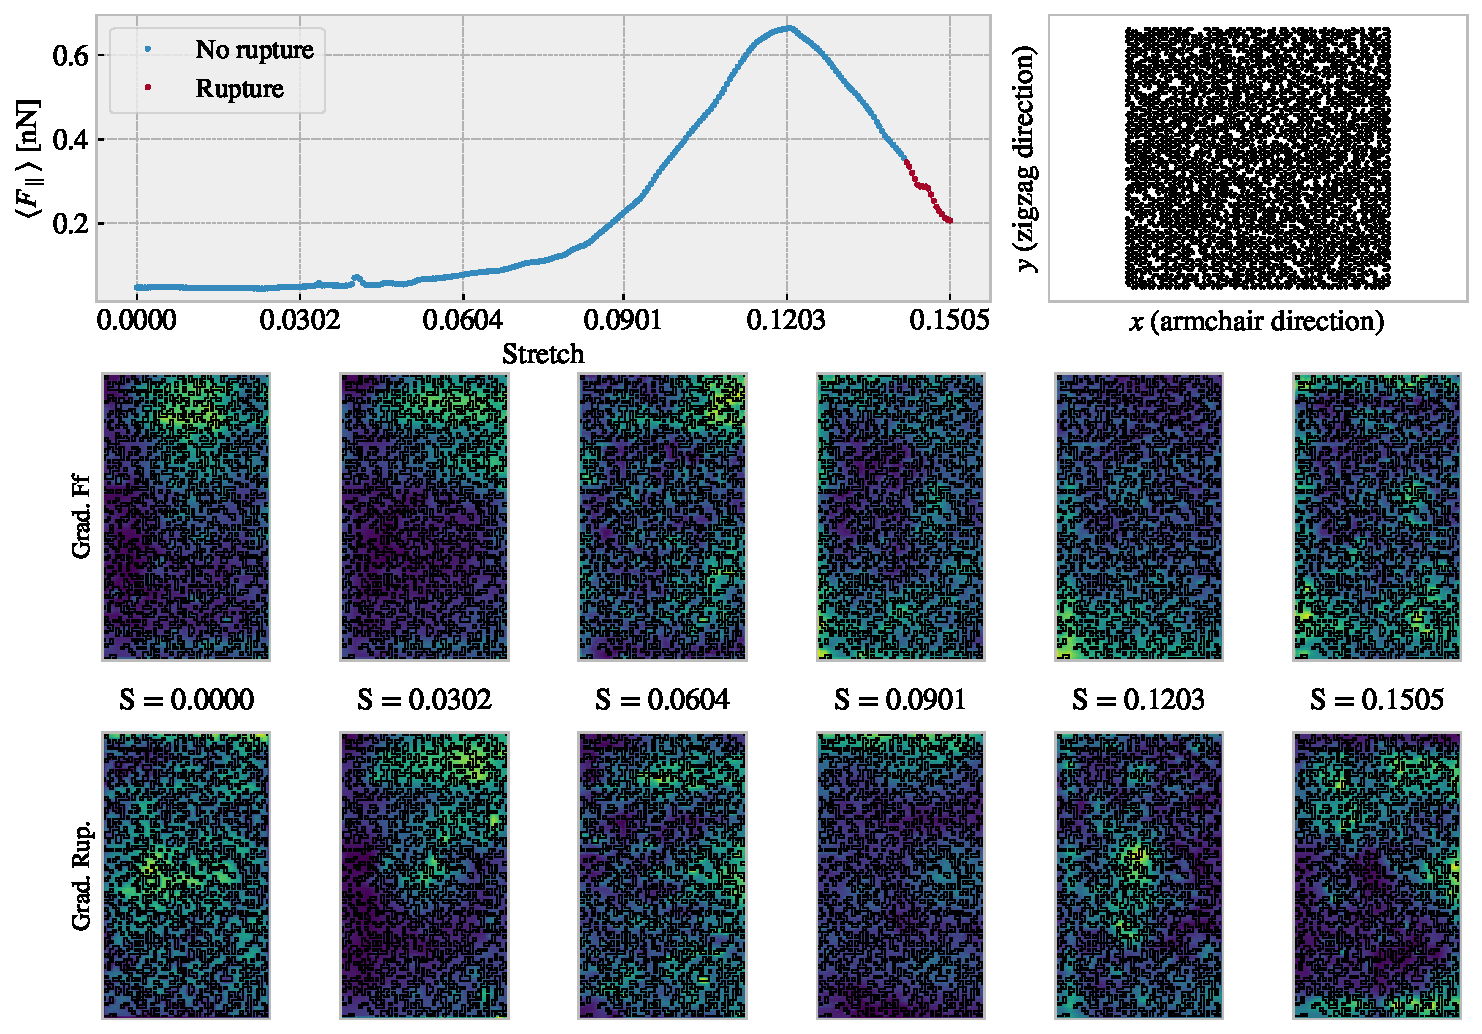
\includegraphics[width=0.75\linewidth]{figures/search/grad_cam_GA_RN_start_top0.pdf}
      \caption{Mixed porosity $p \in \{0.01, 0.05, 0.1, 0.2, 0.3\}$.}
      % \caption{}
      \label{fig:GC_mixed_p}
  \end{subfigure}
  \hfill
  \vspace{1cm}
  \begin{subfigure}[t]{1\textwidth}
      \centering
      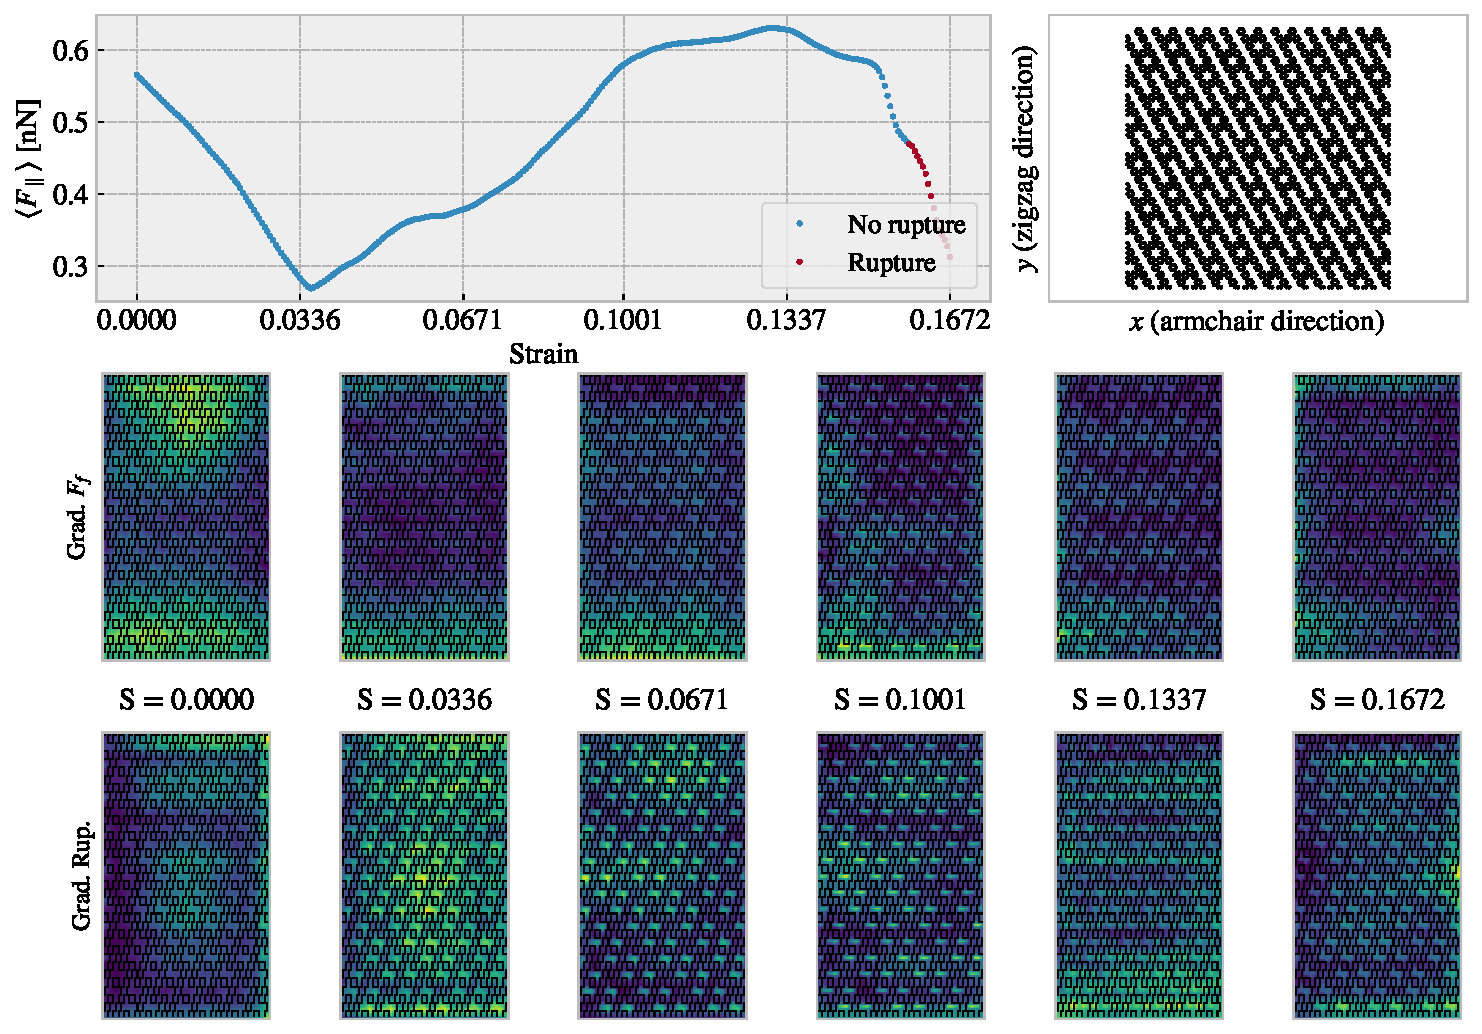
\includegraphics[width=0.75\linewidth]{figures/search/grad_cam_pop_1_7_1_1_4.pdf}
      \caption{Tetrahedron $(1,7,1)$, ref = $(1,4)$.}
      % \caption{}
      \label{fig:GC_pop_search}
  \end{subfigure}
  \hfill
  \caption{(The figure continues on the next page)}
\end{figure}

\begin{figure}[!htb]\ContinuedFloat
  \centering
  \begin{subfigure}[t]{1\textwidth}
      \centering
      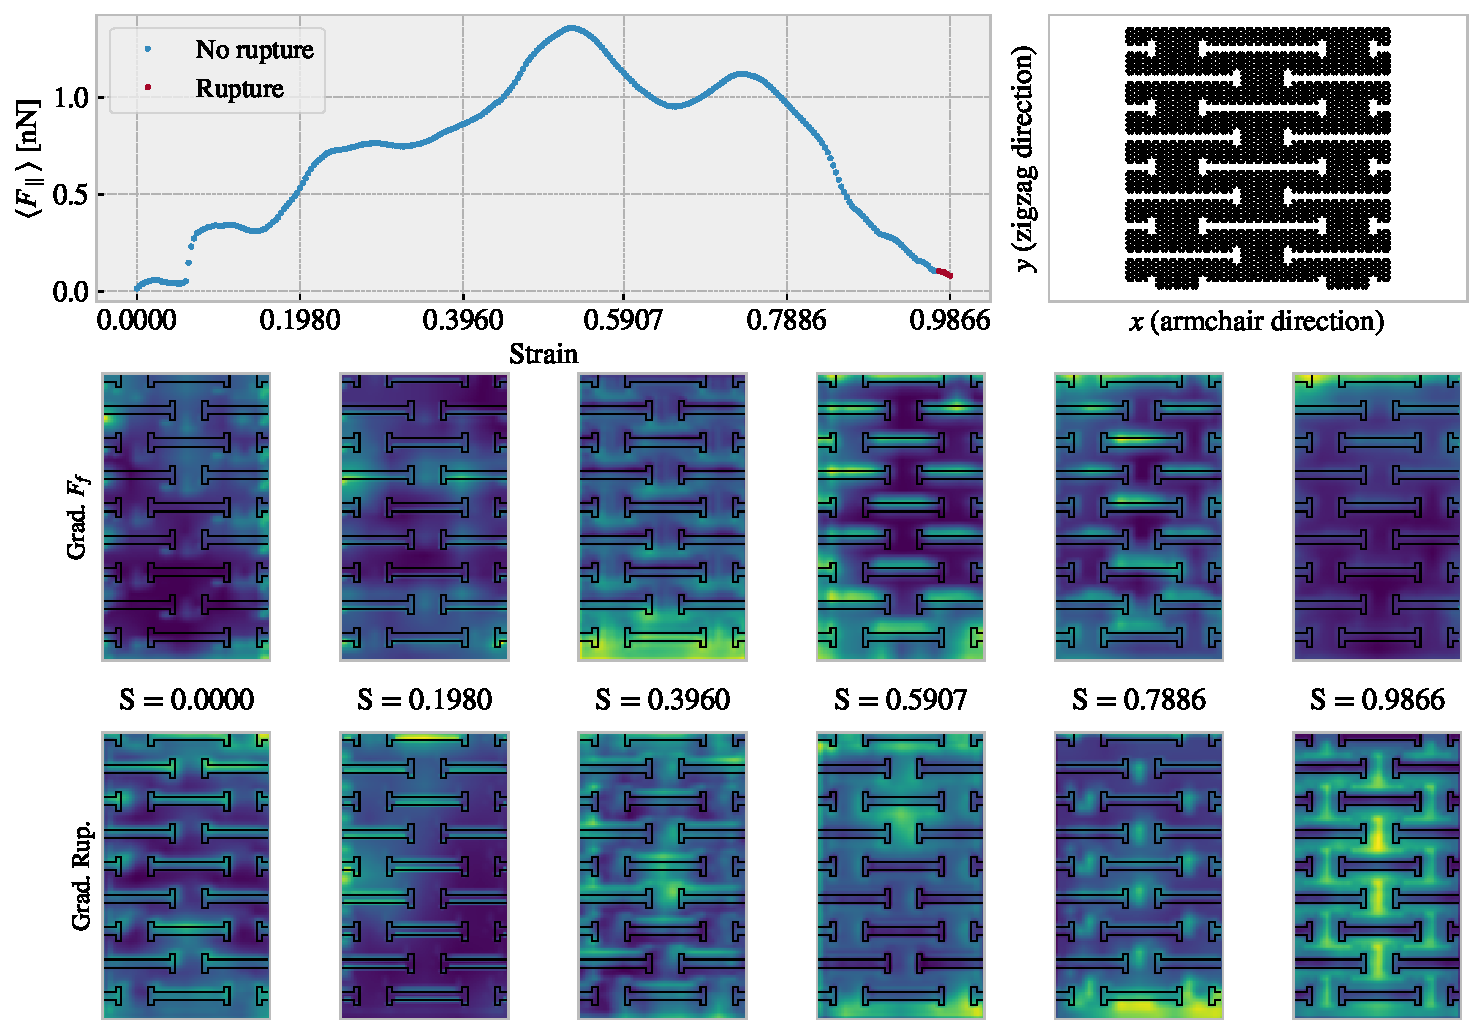
\includegraphics[width=0.75\linewidth]{figures/search/grad_cam_hon_3_3_5_3_12_0.pdf}
      \caption{Honeycomb $(3,3,5,3)$, ref = $(12,0)$.}
      % \caption{}
      \label{fig:GC_hon_search}
  \end{subfigure}
  \hfill
  \vspace{5mm}
  \begin{subfigure}[t]{1\textwidth}
    \centering
    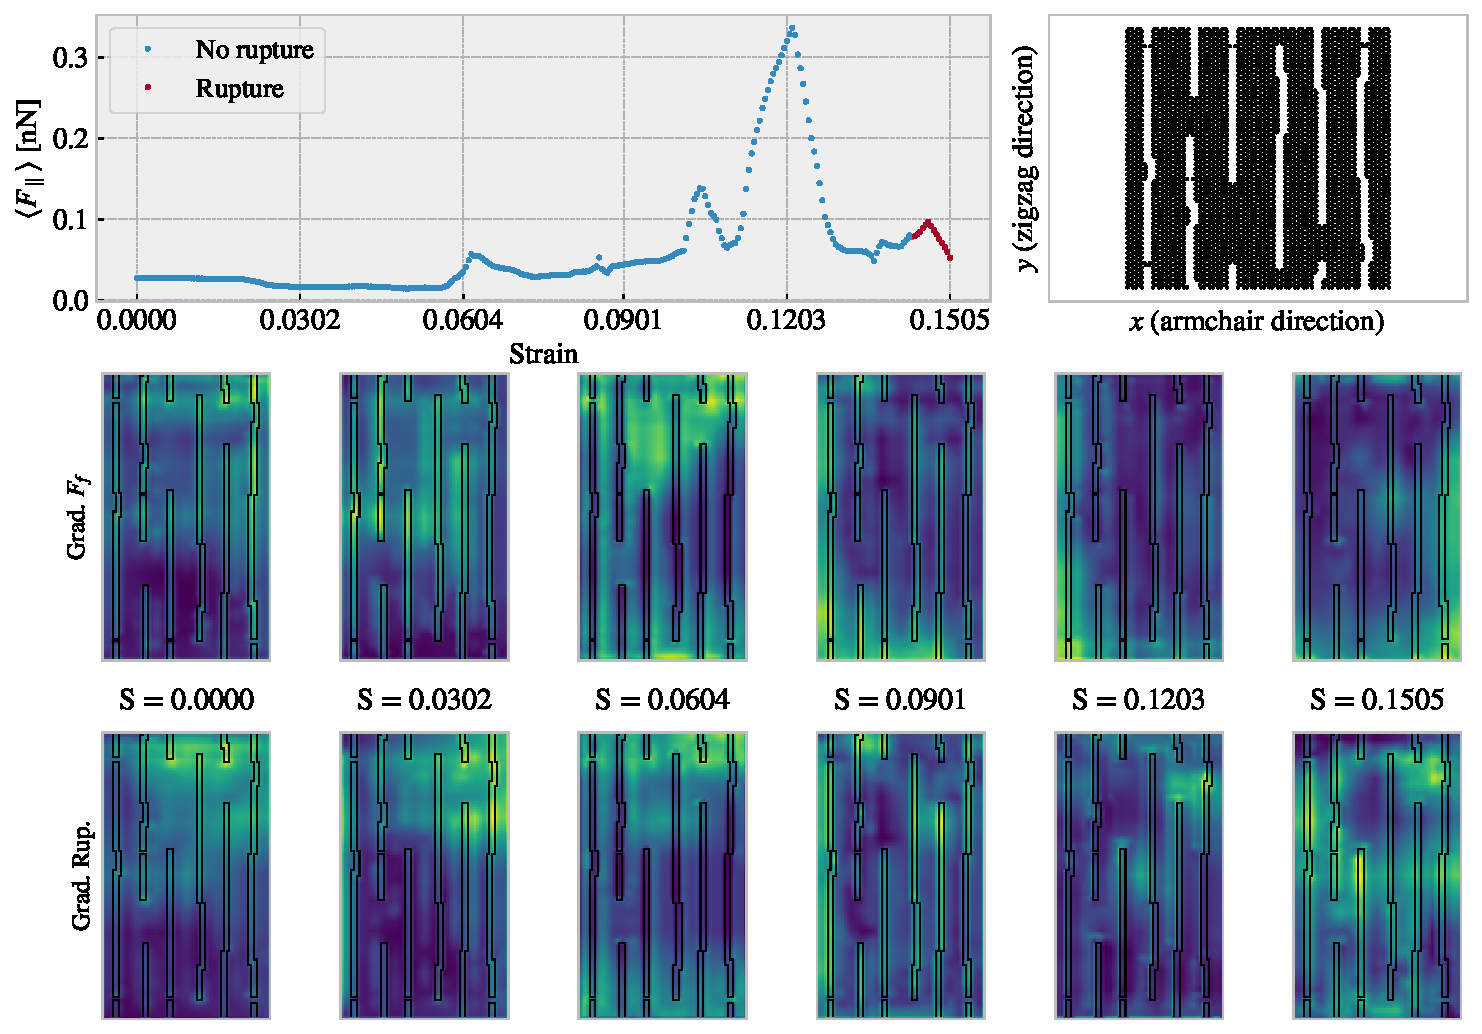
\includegraphics[width=0.75\linewidth]{figures/search/grad_cam_RW_search_max_drop0.pdf}
    \caption{Random walk.}
    % \caption{}
    \label{fig:GC_RW_search}
\end{subfigure}
\hfill
  \caption{Grad-CAM analysis of selected Kirigami configurations. The top row
  shows the predicted friction-strain curve (left) with the rupture prediction
  indicated by the colors (blue: no rupture, red: rupture), and a visualization
  of the Kirigami graphene sheet on the hexagonal lattice (right). The remaining
  rows show the grad-CAM heatmaps with respect to the prediction of the friction
  (Grad.\ $F_f$) and rupture (Grad.\ rup) respectively, for various strain values
  corresponding to the x-axis ticks on the friction-strain curve. The edges of the cut patterns are marked with black lines for reference. The four
  configurations displayed are: (a) The top-scoring individual from the genetic
  algorithm search using a mixed porosity start. (b) The Tetrahedron $(1,7,1)$
  with a reference point $(1,4)$ which gave the highest max drop score in the
  investigation of pattern translation in~\cref{fig:tetra_171_trans}. (c) The
  Honeycomb $(3,3,5,3)$ with a reference point $(12,0)$ which gave the highest
  max drop score in the investigation of pattern translation
  in~\cref{fig:hon_3353_trans}. (d) The highest scoring candidate for the max drop property in the Random walk pattern generation search shown in~\cref{fig:RW_search_top5}. }
  \label{fig:grad_cam}
\end{figure}


